\documentclass[
oneside,
a4paper,
12pt,
titlepage]
{article}
\usepackage[english]{babel}

% \usepackage[LANGUAGE]{babel} % must be set in a per-file manner
\usepackage[utf8]{inputenc}
\usepackage{graphicx} % notwendig für das Einbetten von Bildern s. http://en.wikibooks.org/wiki/LaTeX/Importing_Graphics
%\usepackage{float} % s. http://tex.stackexchange.com/questions/119799/text-next-to-image
\usepackage{amsmath}
\usepackage{amssymb}
\usepackage{fontspec}
\usepackage{unicode-math}
\usepackage{caption}
\usepackage{geometry}
\usepackage{booktabs}
\usepackage{tabularx} % notwendig für Zeilenumbruch in Tabellenzelle http://tex.stackexchange.com/questions/2441/how-to-add-a-forced-line-break-inside-a-table-cell
\usepackage{longtable}
\usepackage{tabu}
\usepackage{multirow}
%\usepackage{fixltx2e} % ermöglicht \textsubscript; verträgt sich nicht mit der [H]-Option von float-Umgebungen
\usepackage{amsthm}
\usepackage{floatrow} % verträgt sich nicht mit float
\usepackage{calc}
\usepackage{setspace} % notwendig zur Festsetzung des Zeilenabstands http://tex.stackexchange.com/questions/74496/how-to-use-times-roman-nimbus-roman-with-fontspec-under-linux-and-lualatex
\usepackage{siunitx} % notwendig für Einheiten in textmode s. http://tex.stackexchange.com/questions/9043/should-greek-letters-inserted-in-text-using-math-mode-mostly-always-be-italic
\usepackage{tikz} % Ermöglicht das Erstellen von Grafiken in LaTeX
\usepackage{circuitikz} % create circuitry
\usepackage{chngcntr} % Ermöglicht das Umschalten von Zählern
\usepackage{paralist} % s.S. 136 Companion
\usepackage{enumitem} % `enumitem´ and `paralist´ seem to conflict
\usepackage{fancyhdr} % aus PFA_woerterbuch.tex
\usepackage{csquotes} % ermöglicht die Verwendung sprachspezifischer Anführungszeichen durch biblatex
\usepackage{textcomp} % um in textmode Minuszeichen schreiben zu können s. http://tex.stackexchange.com/questions/24423/writing-a-negative-number-in-text-mode-9-or-9
\usepackage{upgreek}
\PassOptionsToPackage{hyphens}{url}
\usepackage{hyperref}
\usepackage[sort]{cleveref}
% \PassOptionsToPackage{hyphens}{url}\usepackage[colorlinks=false]{hyperref} % s.S. 50 biblatex-Dokumentation und http://tex.stackexchange.com/questions/3033/forcing-linebreaks-in-url
% \usepackage{url} % probably not necessary, since `url´ is loaded by `hyperref´
\usepackage{commath}
\usepackage{pdflscape}
\usepackage{listings}  %% For inserting and syntax highlighting source code files.
%% \usepackage{minted}  %% For inserting and syntax highlighting source code files.
\usepackage{tracklang}  %% Required by package "datetime2".
\usepackage{datetime2}  %% For inserting dates and times in different formats.
\usepackage{interval}

%%% Local Variables:
%%% mode: latex
%%% TeX-master: "../MasArThesis.tex"
%%% End:

% This file contains both package specific and LaTeX-internal settings;
% `package specific´ means every setting related to the respective package, even if the setting is done via LaTeX primitives (e.g., `\setcounter´)
% `LaTeX-internal´ means only those settings, which cannot be attributed to a specific package;
% CONVENTIONS:
% -comments ought to be placed on the line on which the command/option they refer to ends 
% -when several options are given in one pair of brackets/curly braces, each one should be separated by a newline character, including the first option)

%%%%%%%%%%%%%%
%% interval %%
%%%%%%%%%%%%%%
\intervalconfig{soft open fences}

%%%%%%%%%%%%%%
%% geometry %%
%%%%%%%%%%%%%%
\geometry{
  % margin=2.5cm % for one-sided documents (this requires `\documentclass[oneside…´)
  margin=2cm,
  inner=3cm,
  % inner=2.5cm, % for two-sided documents (this requires `\documentclass[twoside…´)
  % outer=3.5cm, % for two-sided documents (this requires `\documentclass[twoside…´)
  a4paper
}

%%%%%%%%%%%%%
%% caption %%
%%%%%%%%%%%%%
\captionsetup{
  font=footnotesize,
  labelfont=bf,
  singlelinecheck=false,
  justification=justified}
  % justification=centering}

%%%%%%%%%%%%%%
%% hyperref %%
%%%%%%%%%%%%%%
\hypersetup{
  colorlinks=false,
  % colorlinks=true,
  linktoc=all}

%%%%%%%%%%%%%%
%% listings %%
%%%%%%%%%%%%%%
\lstset{
  basicstyle=\ttfamily,
  keywordstyle=,
  showstringspaces=false}

%%%%%%%%%%%%%%
%% setspace %%
%%%%%%%%%%%%%%
% \singlespacing
\onehalfspacing
% \doublespacing

%%%%%%%%%%%%%%
%% enumitem %%
%%%%%%%%%%%%%%
\setlist[itemize]{
  topsep=0cm,
  partopsep=0cm,
  itemsep=0cm} % s. p. 9 enumitem

%%%%%%%%%%%%%%
%% tabularx %%
%%%%%%%%%%%%%%
\newcolumntype{C}{>{\centering\arraybackslash}X}
\newcolumntype{L}{>{\raggedright\arraybackslash}X}
\newcolumntype{R}{>{\raggedleft\arraybackslash}X}

%%%%%%%%%%%%%%
%% paralist %%
%%%%%%%%%%%%%%
\setdefaultitem{\textendash}{\textbullet}{$\square$}{}

%%%%%%%%%%%%%%
%% fontspec %%
%%%%%%%%%%%%%%
% \setmainfont{TeX Gyre Termes}
\setmainfont{XITS}

%%%%%%%%%%%%%%%%%%
%% unicode-math %%
%%%%%%%%%%%%%%%%%%
\setmathfont[
math-style=ISO,
bold-style=literal,
% vargreek-shape=TeX  %% Obsolote as of v0.8d (see https://ctan.org/ctan-ann/id/mailman.2585.1485610970.17497.ctan-ann@ctan.org)
]{XITS Math}

%%%%%%%%%%%%%%
%% floatrow %%
%%%%%%%%%%%%%%
\floatsetup[table]{
  style={plaintop},
  font={normalsize}}
  % font={scriptsize}} %% this setting for some reason affected the longtabu environment, but not the tabu environment
\floatsetup[figure]{capposition=bottom}
\newfloatcommand{myffigbox}{figure}[][\myimagewidth]
\newfloatcommand{mykarte}{figure}[][\textwidth]

%%%%%%%%%%%%%
%% siunitx %%
%%%%%%%%%%%%%
\sisetup{
  locale = US, % manages the locale specific display of numbers, SI units, etc.
  % locale = DE,
  list-final-separator = {, and },
  exponent-product = \cdot,
  redefine-symbols = false, % s. p. 62 siunitx
  group-minimum-digits = 3,
  group-digits = integer,
  table-text-alignment = center,
  table-number-alignment = center
}

%%%%%%%%%%%%%%%
%% longtable %%
%%%%%%%%%%%%%%%
\setcounter{LTchunksize}{10}

%%%%%%%%%%%%%%%%%%%%%%%%%%%%%%%%
%% LaTeX: lengths, skips, etc %%
%%%%%%%%%%%%%%%%%%%%%%%%%%%%%%%%
\setlength{\parindent}{0 cm} % indentation of paragraphs
\setlength{\parskip}{10 pt} % extra vertical space between paragraphs; s. p. 2 “Formatvorlage-Waldökosystemmanagement.doc”: “Nach”
\newlength{\myabovetop}
\setlength{\myabovetop}{2\baselineskip}
\newlength{\myimagewidth}
\setlength{\myimagewidth}{5.65cm}
\newlength{\capskip}
\setlength{\capskip}{-0.35cm}
\setlength{\abovecaptionskip}{0.5\baselineskip}
\setlength{\belowcaptionskip}{0.5\baselineskip}

%%%%%%%%%%%%%%%%%%%%%%%%%
%% LaTeX: environments %%
%%%%%%%%%%%%%%%%%%%%%%%%%
\newenvironment{mytable}[2]{\begin{table}[htb]\scriptsize\caption{#1\vspace{\capskip}}\label{#2}}{\end{table}\par} % \vspace notwendig wegen floatrow

%%%%%%%%%%%%%%%%%%%%%
%% LaTeX: counters %%
%%%%%%%%%%%%%%%%%%%%%
\setcounter{topnumber}{2} % s. p. 284 ff. Companion
\setcounter{bottomnumber}{1} % s. p. 284 ff. Companion
\setcounter{totalnumber}{3} % s. p. 284 ff. Companion
\setcounter{figure}{0}

%%% Local Variables:
%%% mode: latex
%%% TeX-master: "../MasArThesis.tex"
%%% End:

% This file contains settings intended for use with documentclass `article´.

%%%%%%%%%%%%%%
%% chngcntr %%
%%%%%%%%%%%%%%
\counterwithout{figure}{section} % counter `figure´ is not reset at the beginning of a new `section´

%%%%%%%%%%%%%%
%% fancyhdr %%
%%%%%%%%%%%%%%
\pagestyle{fancy}
\fancyhead{}
\fancyfoot{}
\fancypagestyle{toc}{ % http://texblog.org/2013/09/16/multiple-page-styles-with-fancyhdr/
\fancyhead{}
\fancyhead[L]{\fontsize{12pt}{1\baselineskip} \selectfont \leftmark \\}
% \fancyhead[R]{\fontsize{10pt}{1\baselineskip} \thepage \\}
\fancyfoot{}
\renewcommand{\footrulewidth}{0.4pt}
\fancyfoot[C]{\fontsize{10pt}{1\baselineskip} \thepage \\}
}
\fancypagestyle{abbrevs_symbols}{ % http://texblog.org/2013/09/16/multiple-page-styles-with-fancyhdr/
\fancyhead{}
\fancyhead[L]{\fontsize{12pt}{1\baselineskip} \selectfont \leftmark \\}
% \fancyhead[R]{\fontsize{10pt}{1\baselineskip} \thepage \\}
\fancyfoot{}
\renewcommand{\footrulewidth}{0.4pt}
\fancyfoot[C]{\fontsize{10pt}{1\baselineskip} \thepage \\}
}
\fancypagestyle{standard}{ % http://texblog.org/2013/09/16/multiple-page-styles-with-fancyhdr/
\fancyhead{}
% \fancyhead[L]{\fontsize{12pt}{1\baselineskip} \selectfont \leftmark \\}
\fancyhead[L]{\fontsize{12pt}{1\baselineskip} \selectfont \firstmark \\}
% \fancyhead[R]{\fontsize{10pt}{1\baselineskip} \thepage \\}
\fancyfoot{}
\renewcommand{\footrulewidth}{0.4pt}
\fancyfoot[C]{\fontsize{10pt}{1\baselineskip} \thepage \\}
}
\fancypagestyle{bibliography}{ % http://texblog.org/2013/09/16/multiple-page-styles-with-fancyhdr/
\fancyhead{}
\fancyhead[L]{\fontsize{12pt}{1\baselineskip} \selectfont \leftmark \\}
% \fancyhead[R]{\fontsize{10pt}{1\baselineskip} \thepage \\}
\fancyfoot{}
\renewcommand{\footrulewidth}{0.4pt}
\fancyfoot[C]{\fontsize{10pt}{1\baselineskip} \thepage \\}
}
\renewcommand{\sectionmark}[1]{%
  \markboth{#1}{}} % s. p. 9 f. fancyhdr
\renewcommand{\subsectionmark}[1]{%
} % to suppress printing of subsection titles in headers (s. `\firstmark´ above)

%%%%%%%%%%%%%%%%%%%%%
%% LaTeX: commands %%
%%%%%%%%%%%%%%%%%%%%%
\renewcommand\topfraction{1.0} % s. p. 284 ff. Companion
\renewcommand\bottomfraction{1.0} % s. p. 284 ff. Companion
\renewcommand\textfraction{0.0} % s. p. 284 ff. Companion 
\renewcommand\floatpagefraction{0.75} % s. p. 284 ff. Companion 
\makeatletter
\renewcommand{\thefigure}{\arabic{figure}}
\renewcommand{\thetable}{\arabic{table}}
\makeatother
\makeatletter
\renewcommand\section{\@startsection
  {section}{1}{0 mm}
  {\myabovetop}
  {0.25\baselineskip}
  {\normalfont\normalsize\bfseries}}
\renewcommand\subsection{\@startsection
  {subsection}{2}{0 mm}
  {\myabovetop}
  {0.25\baselineskip}
  {\normalfont\normalsize\itshape}}
\renewcommand\subsubsection{\@startsection
  {subsubsection}{2}{0 mm}
  {0 pt}
  {0.05\baselineskip}
  {\normalfont\normalsize}}
\makeatother

%%% Local Variables:
%%% mode: latex
%%% TeX-master: "../MasArThesis.tex"
%%% End:

\usepackage[
backend=biber,
% bibstyle=/home/renke/Uni/Formatvorlagen/LaTeX/BibstylePapers,
bibstyle=authoryear,
% citestyle=/home/renke/Uni/Formatvorlagen/LaTeX/CitestylePapers,
citestyle=authoryear-comp,
natbib=false,
mcite=false,
sorting=nyt,
sortcase=false,
sortcites=true,
maxbibnames=99,
maxcitenames=2,
maxitems=2,
uniquename=false,
autocite=plain,
language=autobib,
hyperref=true,
urldate=long,
dateabbrev=false,
date=year,  % cp. https://tex.stackexchange.com/questions/55780/disable-month-in-biblatex-bibliography
giveninits=true,
bibencoding=utf8 % s. p. 42 ff. biblatex
]{biblatex} % s. p. 45 ff. biblatex

% \addbibresource[location=local]{../../Literatur/MODULNAME} % s. p. 71 f. biblatex; must be set in a per-file manner

\renewcommand*{\nameyeardelim}{\space} % http://tex.stackexchange.com/questions/134063/how-to-add-a-comma-between-author-and-year
\renewcommand*{\revsdnamepunct}{\space}
\renewcommand*{\finentrypunct}{}
\renewcommand*\finalnamedelim{%
  \ifnumgreater{\value{liststop}}{2}{\addspace\bibstring{and}\addspace}%
  {\addspace\biband\addspace}}% http://tex.stackexchange.com/questions/67621/biblatex-have-and-in-the-citation-but-in-the-bibliography

\renewbibmacro*{doi+eprint+url}{%  https://tex.stackexchange.com/questions/154864/biblatex-use-doi-only-if-there-is-no-url
\iftoggle{bbx:url} {\iffieldundef{doi}{\usebibmacro{url+urldate}}{}} {}%
\newunit\newblock \iftoggle{bbx:eprint} {\usebibmacro{eprint}} {}%
\newunit\newblock \iftoggle{bbx:doi} {\printfield{doi}} {}}

\DeclareNameAlias{sortname}{last-first} % http://tex.stackexchange.com/questions/12806/guidelines-for-customizing-biblatex-styles/13076#13076

\DeclareNosort{} % http://tex.stackexchange.com/questions/171492/biblatex-biber-is-incorrectly-sorting-entries-with-hyphens-in-their-respective-a
\DeclareNoinit{
  \noinit{\regexp{[\x{2bf}\x{2018}]}}} % http://tex.stackexchange.com/questions/171492/biblatex-biber-is-incorrectly-sorting-entries-with-hyphens-in-their-respective-a

\newcommand{\biband}{\ifcurrentname{labelname}{\addspace \& \addspace}{\addspace \addcomma \addspace}} % http://tex.stackexchange.com/questions/67621/biblatex-have-and-in-the-citation-but-in-the-bibliography

%%% Local Variables:
%%% mode: latex
%%% TeX-master: "../MasArThesis.tex"
%%% End:

\hyphenation{li-mi-ting}
\hyphenation{sev-er-al}
\hyphenation{ag-ri-cul-tur-al}

%%% Local Variables:
%%% mode: latex
%%% TeX-master: "../MasArThesis.tex"
%%% End:

\hyphenation{zu-zu-schrei-ben}
\hyphenation{Ge-bie-te}
\hyphenation{Wunsch-er-fül-lung}
\hyphenation{der-ar-ti-ge}
\hyphenation{be-stim-mten}
\hyphenation{be-stim-mte}
\hyphenation{mo-ra-li-sche}
\hyphenation{mo-ra-li-schem}
\hyphenation{mo-ra-li-schen}
\hyphenation{mo-ra-li-scher}
\hyphenation{mo-ra-li-sches}
\hyphenation{Un-rechts-er-eig-nis}
\hyphenation{Rechts-an-sprü-chen}
\hyphenation{Rechts-an-sprü-che}
\hyphenation{Rechts-an-spruch}
\hyphenation{re-le-vant}
\hyphenation{Re-le-vanz}
\hyphenation{Rah-men-be-ding-ung-en}
\hyphenation{fort-ge-setz-ten}
\hyphenation{fort-ge-setzt}
\hyphenation{Ein-tref-fen}
\hyphenation{Ein-tref-fens}
\hyphenation{Le-bens-chan-cen}
\hyphenation{Le-bens-chan-ce}
\hyphenation{mensch-lich-es}
\hyphenation{mensch-lich}
\hyphenation{mensch-lich-er}
\hyphenation{mensch-lich-en}
\hyphenation{Be-schrän-kung}
\hyphenation{Täu-schung}
\hyphenation{be-tref-fen}
\hyphenation{stell-ver-tre-tend}
\hyphenation{Ge-rech-tig-keits-an-sprüche}
\hyphenation{Un-rechts-zu-stand}
\hyphenation{zwi-schen}
\hyphenation{Pflich-ten}
\hyphenation{un-glei-chen}
\hyphenation{mei-nen}
\hyphenation{Eigen-tums-rechts}
\hyphenation{Eigen-tums-recht}
\hyphenation{Rech-ten}
\hyphenation{zu-sätz-li-cher}
\hyphenation{schlech-ten}
\hyphenation{Nicht-i-den-ti-täts-pro-blem}
\hyphenation{Pro-blem}
\hyphenation{zu-kunfts-o-ri-en-tiert}
\hyphenation{be-sei-ti-gen-den}
\hyphenation{Ei-gen-tums-rech-ten}
\hyphenation{Fa-kul-tät}
\hyphenation{For-schungs-an-stal-ten}
\hyphenation{Mo-del-lie-rung}
\hyphenation{Ver-suchs-an-stalt}
\hyphenation{Durch-mes-ser}
\hyphenation{er-trags-kund-licher}
\hyphenation{grund-flä-chen-ge-steu-er-ten}

%%% Local Variables:
%%% mode: latex
%%% TeX-master: "../MasArThesis.tex"
%%% End:


%% Input settings files specific to this document.
\input{TikZSettings.tex}

\addbibresource[location=local]{../../Literature/MasAr_Literature.bib} % s. S. 71 f. biblatex-Dokumentation

%% AUCTeX style file: ./style/MasArThesis.el

%% Define custom SI units.
\DeclareSIUnit\year{a}

%% Define custom commands/math operators (in alphabetical order). Note: command names may not contain non-letters.
\newcommand{\BasalAreaR}{\texttt{G}}
% \newcommand{\Beech}[0]{European beech (\emph{Fagus sylvatica} L.)}
\newcommand{\Beech}[0]{beech}
\DeclareMathOperator{\diag}{diag}
\newcommand{\edf}{effective degrees of freedom}
\DeclareMathOperator{\erf}{erf}
\newcommand{\gamlssPackageVersion}{5.0.4}
\newcommand{\gamlssdistPackageVersion}{5.0.3}
\newcommand{\loglikelihood}{\ell}
\newcommand{\logNlogDcurve}{log(\(N\))-log(\(D\))-curve}
\newcommand{\mgcvPackageVersion}{1.8.22}
\newcommand{\NWFVA}{Northwest German Forest Research Institute}
\newcommand{\Ponderosa}[0]{Ponderosa pine (\emph{Pinus ponderosa} \textsc{Douglas})}
\newcommand{\ProductivityIndexMath}{PI}
\newcommand{\ProductivityIndexText}{absolute productivity index of stand}
\newcommand{\ProductivityIndexVariableMath}{PI_{\text{diff}}}
\newcommand{\ProductivityIndexVariableR}{\texttt{PIV}}
\newcommand{\ProductivityIndexVariableText}{productivity index variable}
\newcommand{\ProductivityIndexYieldClassIMath}{PI_{\text{I. YC}}}
\newcommand{\scamPackageVersion}{1.2.2}
\newcommand{\SeePage}[1]{(see page \pageref{#1})}
\newcommand{\SeeSection}[1]{(see section \ref{#1})}
\DeclareMathOperator{\sign}{sign}
% \newcommand{\Spruce}{Norway spruce (\emph{Picea abies} (L.) H.\textsc{Karst})}
\newcommand{\Spruce}{spruce}
\newcommand{\StandAgeVariableMath}{h_{100}(x)_{\text{YC 1}}}
\newcommand{\StandAgeVariableR}{\texttt{SAV}}
\newcommand{\statsPackageVersion}{3.3.3}
\newcommand{\SterbadgGmaxMath}{d_{g \SterbaGmaxMath{}}}
\newcommand{\SterbaGmaxMath}{G_{max}}
\newcommand{\SterbaNGmaxMath}{N_{\SterbaGmaxMath{}}}
\newcommand{\TopHeightMath}{h_{100}}
\DeclareMathOperator{\tr}{tr}

\begin{document}

\begin{titlepage}

\begin{center}

\vspace*{5cm}

{\LARGE Modeling maximum basal area of pure beech and spruce stands in northwestern Germany \\}

\vspace{2cm}

{\large Author: \\ Renke Christian von Seggern \par}

\vspace{2cm}

{\normalsize Master’s Thesis at the \\
  Faculty of Forest Sciences and Forest Ecology, \\
  Georg-August-Universität Göttingen}

\vspace{0.5cm}

{\normalsize Date of submission: \\ December 20, 2017 \par}

\vspace{0.5cm}

{\normalsize Supervisors: \\ Prof. Dr. Winfried Kurth \\ Prof. Dr. Jürgen Nagel \par}

\end{center}

\end{titlepage}

%%% Local Variables:
%%% mode: latex
%%% TeX-master: "MasArThesis.tex"
%%% End:

\newpage

\input{ToC.tex}
\newpage

\pagestyle{abbrevs_symbols}

{
  \renewcommand{\MakeUppercase}[1]{#1} % http://tex.stackexchange.com/questions/179966/fancyhdr-chaptermark-and-table-of-contents

  \newcommand{\mysectiontitle}{Table of abbreviations and symbols} % set section title as a custom macro to ease mutlitple usage (necessary when using a starred sectioning macro)
  
  \section*{\mysectiontitle{}}
  \label{sec:AbbrevsSymbolsTable}
  
  \markboth{\mysectiontitle{}}{} % http://tex.stackexchange.com/questions/89914/chapter-name-in-the-header-with-chapter
  \addcontentsline{toc}{section}{\mysectiontitle{}} % http://tex.stackexchange.com/questions/35433/creating-unnumbered-chapters-sections-plus-adding-them-to-the-toc-and-or-header
  
  % \begin{table}[H]
  %   \centering
  \begin{longtabu}{l L l}
    \toprule
    Symbol & Description & Unit \\
    \midrule
    \endfirsthead
    Symbol & Description & Unit \\
    \midrule
    \endhead
    \bottomrule
    \endlastfoot
    \(CV(\uplambda)\) & cross validation sum of squares for smoothing parameter \(\uplambda\) \\
    \(D\) & average diameter (by basal area) & \si{\centi\meter} \\
    \(\diag(\symbf{x})\) & diagonal matrix with main diagonal \(\symbf{x}\) \\
    \(\erf\) & error function \\
    \(\exp\) & exponential function \\
    \(\mathbb{E}(x)\) & expectation of variable \(x\) \\
    \(G\) & basal area & \si{\square\meter} \\
    GAM & generalized additive model & \\
    GAMLSS & generalized additive model for location, scale, and shape \\
    GCV & generalized cross validation & \\
    \(GCV(\uplambda)\) & generalized cross validation sum of squares for smoothing parameter \(\uplambda\) \\
    GLM & generalized linear model & \\
    \(\TopHeightMath{}\) & top height, height of dominant trees & \si{\meter} \\
    \(\StandAgeVariableMath{}\) & stand age variable (top height at age \(x\) if the stand were yield class \num{1}) & \si{\meter} \\
    % \(k\) & constant (varying with species) & \\
    \(\loglikelihood(x)\) & log-likelihood of \(x\) \\
    LM & Linear Model & \\
    \(\ln\) & natural logarithm \\
    \(\log\) & decadic logarithm \\
    \(N\) & stand density & \si{\per\hectare} \\
    % \(s\) & slope of the \logNlogDcurve{} \\
    \(\ProductivityIndexMath\) & \ProductivityIndexText{} (\(\TopHeightMath{}\) at age \SI{100}{\year}) & \si{\meter} \\
    SCAM & shape constrained additive model \\
    \(\sign\) & sign function \\
    \(\tr(\symbf{A})\) & trace of square matrix \(\symbf{A}\) \\
    % UBRE & un-biased risk estimator \\
  \end{longtabu}
  % \end{table}
}

%% Reset table counter.
\setcounter{table}{0}

%%% Local Variables:
%%% mode: latex
%%% TeX-master: "MasArThesis.tex"
%%% End:

\newpage

\section*{Zusammenfassung}
{
  \newcommand{\mysectiontitle}{Zusammenfassung} % set section title as a custom macro to ease mutlitple usage (necessary when using a starred sectioning macro)
  \markboth{\mysectiontitle{}}{} % http://tex.stackexchange.com/questions/89914/chapter-name-in-the-header-with-chapter

  \fancypagestyle{zusammenfassung}{ % http://texblog.org/2013/09/16/multiple-page-styles-with-fancyhdr/
    \fancyhead{}
    % \renewcommand{\headrulewidth}{0pt}
    \fancyhead[L]{\fontsize{12pt}{1\baselineskip} \selectfont \leftmark \\}
    \fancyfoot{}
    % \renewcommand{\footrulewidth}{0pt}
    \fancyfoot[C]{\fontsize{10pt}{1\baselineskip} \thepage \\}
  }
  \pagestyle{zusammenfassung}

  Die maximale oder natürliche Bestandesgrundfläche ist eine vielseitig einsetzbare Größe und kann beispielsweise als Referenz zur Bestimmung von Durchforstungsstärken dienen.  Sie lässt sich jedoch nur auf Nullgrad-Dauerversuchsflächen zweifelsfrei bestimmen, wobei derartig ermittelte Werte streng genommen nur auf Bestände vergleichbarer Produktivität übertragbar sind.  Da derartige Versuchsflächennur in begrenztem Umfang vorhanden sind, muss auf andere Methoden der Grundflächenermittlung zurückgegriffen werden.  Hierfür bieten sich statistische Modelle an.  Die Auswahl derartiger Modelle ist allerdings eng begrenzt. Insbesondere fehlt es bisher an einer Möglichkeit, die maximale Bestandesgrundfläche unter Berücksichtigung von Unterschieden in der Bestandesproduktivität modellieren.  Diese Arbeit zielt darauf ab, diese Lücke zu schließen.  Zur Anwendung kommen generalisierte additive Modelle (GAMs), formeingeschränkte additive Modelle (SCAMs) sowie generalisierte additive Modelle für Lage, Skalierung und Form (GAMLSSs).  All diese Modelltypen stellen eine Erweiterung generalisierter linearer Modelle (GLMs) dar.  Im Gegensatz zu letzteren bieten sie eine höhere Flexibilität.  Insbesondere sind GAMLSSs nicht auf Wahrscheinlichkeitsverteilungen der Exponentialfamilie beschränkt und gestatten die unmittelbare Schätzung nicht nur des Lageparameters, sondern aller jeweiligen Verteilungsparameter.  Diese erhöhte Flexiblität bringt jedoch eine weniger intuitive Interpretation der Modellergebnisse mit sich.
  
  Um sicherzustellen, dass ein Modell \emph{maximale} Bestandesgrundflächen vorhersagt, sollte dieses mithilfe von Daten angepasst werden, die ihrerseits in Beständen mit wenigstens näherungsweise maximaler Bestandesgrundfläche erhoben wurden.  Eine Möglichkeit zur Gewinnung derartiger Daten besteht darin, sie aus einem größeren Datensatz auszuwählen.  Als Auswahlkriterium wird in der vorliegenden Arbeit die Steigung in der von \textcite{Reineke1933} aufgestellten Gleichung verwendet, die mit artspezifischen Steigungen von Beständen verglichen wird, in denen Selbstdurchforstung stattfindet.
  
  Es werden insgesamt 6 Modelle an je einen Buchen- und einen Fichtendatensatz aus Nordwestdeutschland angepasst.  Es kann gezeigt werden, dass eine Einschränkung der Modellflexibilität einerseits zu plausibleren Ergebnissen, andererseits aber zu einer verringerten Aussagekraft in Gestalt höherer AIC-Werte führt.  Mögliche Schwächen der zugrundeliegenden Datensätze und ihre Auswirkung auf die Anwendbarkeit der Modelle werden diskutiert.  Die erlangten Modelle werden mit bereits vorhandenden Ansätzen zur Modellierung maximaler Bestandesgrundflächen verglichen.

  
}
%%% Local Variables:
%%% mode: latex
%%% TeX-master: "MasArThesis.tex"
%%% End:


\pagestyle{standard}
\pagenumbering{arabic}

\newpage
\section{Introduction}

\section*{}
% \subsubsection*{}
\begin{frame}[c]
  \only<\theFirstElement>{}
\end{frame}

\section{Einleitung}
\subsection{Ziel, Probleme, Lösungsansätze}
\begin{frame}[c]
  \begin{itemize}
  \item<\theFirstElement-> Ziel: \\
    Modellierung der \emph{maximalen} Bestandesgrundfläche in Abhängigkeit von \emph{Alter} und \emph{Bonität} gleichaltriger Buchen- und Fichtenreinbestände
  \item<\theSecondElement-> Probleme:
    \begin{itemize}
    \item<\theSecondElement-> Trainingdatensatz muss von maximalbestockten Flächen stammen
    \item<\theSecondElement-> Direkt messbare Variablen (z.B. \(h_{100}\)) als Prädiktoren ungeeignet, da sie Alters- und Bonitätseffekte enthalten
    \item<\theSecondElement-> Gängige Modelle erscheinen unzureichend
    \end{itemize}
  \end{itemize}
  \begin{itemize}
  \item<\theThirdElement-> Lösungsansätze:
    \begin{itemize}
    \item<\theThirdElement-> Auswahl der Trainingdaten anhand der Mortalitätsrate
    \item<\theThirdElement-> Trennung von Alters- und Bonitätseffekten
    \item<\theThirdElement-> GAM (Generalized Additive Model) und GAMLSS (Generalized Additive Model for Location, Scale and Shape)
    \end{itemize}
  \end{itemize}
\end{frame}

%%% Local Variables:
%%% mode: latex
%%% TeX-master: "MasArPresentation.tex"
%%% End:


\section{Material and Methods}
\section{Auswahl der Daten}
\subsection{Reineke-Gleichung}
\begin{frame}[c]
  \visible<\theFirstElement->{
    \begin{center}
      \begin{minipage}{0.40\textwidth}
        \centerline{\(\mylog(N) = \textcolor{red}{s} \log(D) + k\)}
        \vspace{\captiondistance}
        \mycaption{Gleichung 1}{Bestandesdichte in Abhängigkeit von mittlerem Durchmesser (Quelle: [1]). \\
          \(N\): Bestandesdichte [\si{\per\hectare}] \\
          \(s\): \textcolor{red}{Steigung} \\
          \(D\): Durchmesser des Grundflächenmittelstammes [\si{\centi\meter}] \\
          \(k\): Konstante (artabhängig)}
      \end{minipage}
    \end{center}

    % \begin{align*}
      % \myscalebox{N} & \myscalebox{: \text{Bestandesdichte [ha\textsuperscript{-1}]}} \\[-3mm]
      % \myscalebox{s} & \myscalebox{: \text{Steigung (}\widehat{=}\text{ \textcolor{red}{Mortalitätsrate})}} \\[-3mm]
      % \myscalebox{D} & \myscalebox{: \text{Durchmesser des Grundflächemittelstammes [cm]}} \\[-3mm]
      % \myscalebox{k} & \myscalebox{: \text{Konstante (artabhängig)}} \\[-3mm]
    % \end{align*}
  }

  \begin{itemize}
  \item<\theSecondElement-> Literatur: \\
    Steigung scheint art- und standortabhängig zu sein (s. z.B. [2])
  \item<\theSecondElement-> Lösungsansatz: \\
    artabhängiger Korridor ,,erlaubter`` Steigungen, begrenzt durch unteren Schwellwert (\(m_u\)) und oberen Schwellwert (\(m_o\))
  \end{itemize}
\end{frame}

\subsection{Auswahlmechanismus}
\begin{frame}[c]
  \begin{columns}
    \begin{column}{0.5\textwidth}
      \visible<\theFirstElement->{
        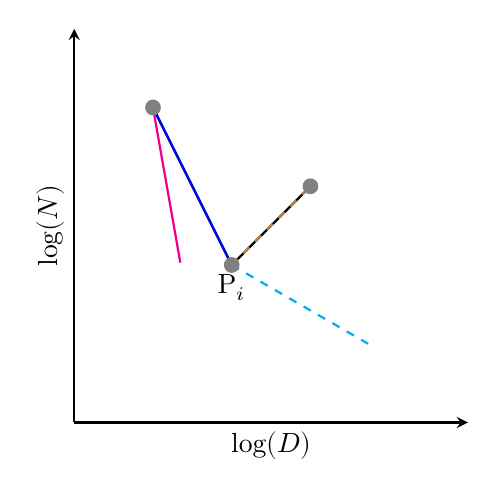
\begin{tikzpicture}[>=stealth]
          %% Coordinate system.
          \draw[black,thick,->] (0,0) -- (5,0);  %% x-axis
          \draw[black,thick,->] (0,0) -- (0,5);  %% y-axis
          \node[anchor=north] at (2.5,0) {\(\log(D)\)};  %% x-axis title
          \node[anchor=south,rotate=90] at (0,2.5) {\(\log(N)\)};  %% y-axis title
          
          %% Specify point coordinates.
          \coordinate (Pi-1) at (1,4);
          \coordinate (Pi) at (2,2);
          \coordinate (Pi+1) at (3,3);

          %% Lines.
          \visible<\theFirstElement-\theSecondElement>{\draw[black,thick] (Pi-1) -- (Pi) -- (Pi+1);}
          \visible<\theSecondElement->{\draw[magenta,thick] (Pi-1) -- ++(280:2cm);}
          \visible<\theSecondElement->{\draw[blue,thick] (Pi-1) -- (Pi);}
          \visible<\theThirdElement->{\draw[cyan,thick,dashed] (Pi) -- ++(330:2cm);}
          \visible<\theThirdElement->{\draw[brown,thick,dashed] (Pi) -- (Pi+1);}

          %% Points.
          \fill[gray] (Pi-1) circle (0.1);
          \fill[gray] (Pi) circle (0.1);
          \fill[gray] (Pi+1) circle (0.1);

          %% Text.
          % \node[anchor=south] at (Pi-1) {\(\text{P}_{i-1}\)};
          \node[anchor=north] at (Pi) {\(\text{P}_i\)};
          % \node[anchor=south] at (Pi+1) {\(\text{P}_{i+1}\)};

        \end{tikzpicture}
        \captionsep{}
        \mycaption{Abbildung 1}{Schematische Darstellung der Funktionsweise des Auswahlmechanismus.}
      }
    \end{column}
    \begin{column}{0.5\textwidth}
      \visible<\theFirstElement->{\(\text{P}_i\) wird ausgewählt, wenn}
      \begin{enumerate}
      \item<\theFirstElement-> es mind. einen benachbarten Punkt gibt (\ding{51}) und
      \item<\theSecondElement-> Steigung \(\textcolor{blue}{s_1} \geq \textcolor{magenta}{m_u}\) (\ding{51}) und
      \item<\theThirdElement-> Steigung \(\textcolor{brown}{s_2} \leq \textcolor{cyan}{m_o}\) (\ding{55}).
      \end{enumerate}
    \end{column}
  \end{columns}
\end{frame}

\subsection{Beispiel: Buche}
\begin{frame}[c]
  \visible<1->{
    \centerline{
      \begin{minipage}{0.9\textwidth}
        \includegraphics[width=1.0\textwidth]{../../Graphics/Presentation/logDlogNPlotsBeforeAfterDataSelectionBeech.pdf}
        \captionsep{}
        \mycaption{Abbildung 2}{Beobachteter Zusammenhang zwischen Bestandesdichte \(N\) und mittlerem Durchmesser \(D\).  Farbige Linien verbinden Beobachtungen eines Bestandes. Gestrichelte bzw. durchgezogene schwarze Linien stellen den oberen bzw. unteren Schwellwert der noch ,,erlaubten`` Steigungen beispielhaft dar. \\
          A: vor Anwendung des Auswahlmechanismus \\
          B: nach Anwendung des Auswahlmechanismus}
      \end{minipage}}}
\end{frame}

%%% Local Variables:
%%% mode: latex
%%% TeX-master: "MasArPresentation.tex"
%%% End:

\subsection{Description of data sets}

The data set size for \Beech{} is reported in \RefTab{tab:ObservationsCountPerEdvidBeech}.  The data set comprises 18 sample plots, with a total of 63 observations and a mean of \num{3.5} observations per sample plot.  The data set size for \Spruce{} is reported in \RefTab{tab:ObservationsCountPerEdvidSpruce}.  The data set comprises 28 sample plots, with a total of 100 observations and a mean of \num{3.6} observations per sample plot.  In both data sets, the number of observations per sample plot ranges from \numrange{2}{8}.

The geographical location and the altitude above sea level of sample plots are reported in \RefFig{fig:LocationsSamplePlots} and \RefFig{fig:SpeciesAltitudeOfSamplePlots}, respectively.  The dots in the plots of both figures do not add up to the total number of sample plots of the respective species because some sample plots were part of the same trial and therefore shared the same geographical location and altitude.  In the \Beech{} data set, altitude above sea level spans \SI{525}{\meter}, ranging from \SIrange{40}{565}{\meter}, with a mean of \SI{313.2}{\meter}.  In the case of \Spruce{} it spans \SI{730}{\meter}, ranging from \SIrange{20}{750}{\meter}, with a mean of \SI{410.5}{\meter}.

In Figures \ref{fig:StandAgeTopHeightYieldClassClassification}, \ref{fig:StandAgeSiteIndexYieldClassClassification}, and \ref{fig:StandAgeBasalAreaYieldClassClassification}, dot color signifies the (fractional) yield class of the respective observation.  Classification of observations into yield classes required multiple steps, which were undertaken separately for each species.  First, for all observations the absolute site index \(SI\) in \si{\meter} was computed using the equation
\begin{equation}
  \label{eq:NagelFunctionSolvedForSI}
  SI = \frac{\TopHeight(x) + 49.872 - 7.3309 \cdot \ln(x) - 0.77338 \cdot \ln(x)^2 }{0.52684 + 0.10542 \cdot \ln(x)} ,
\end{equation}
\parencite{Nagel1999} where \(x\) is stand age and \(\TopHeight(x)\) is top height in \si{\meter} at age \(x\).  Next, a sequence of \(\TopHeight{}\)-values at age \SI{100}{\year} was generated, ranging from yield class \num{4} to yield class \num{-2}, using an increment of \SI{0.1}{\meter}, thus also covering fractional yield classes.  Values for yield classes \numrange{4}{1} were taken from \textcite{Schober1995} for moderately thinned stands of the respective species, while values for yield classes \numrange{0}{-2} were linearly interpolated from those for yield classes \numlist{2; 1}.   This sequence was then restricted to the range between the best yield class needed to include the lowest observed \(SI\) and the worst yield class needed to include the highest observed \(SI\).  A color palette matching this restricted sequence was then generated, ranging from red (worst yield class observed) over yellow and green to blue (best yield class observed).  Each observed \(SI\) was then mapped to the color representing the corresponding \(\TopHeight{}\)-value.  Considering \RefFig{fig:StandAgeTopHeightYieldClassClassification}, the method of yield class classification yielded plausible results in both data sets:  for a given top height, yield class gradually worsens as stand age increases.

As can be seen from \RefFig{fig:StandAgeTopHeightYieldClassClassification}, several differences between the \Beech{} data set and the \Spruce{} data set exist.  In the former, stands are notably older and cover a wider range of ages, with stand age ranging from \SIrange{35}{153.6}{\year} (difference: \SI{118.6}{\year}), whereas in the latter it ranges from \SIrange{15}{113}{\year} (difference: \SI{98}{\year}).  Consequently, stands in the \Beech{} data set have a higher top height, with \(\TopHeight\) ranging from \SIrange{16.3}{39.2}{\meter} (difference: \SI{22.9}{\meter}), but \Spruce{} stands cover a slightly wider range of top heights, with \(\TopHeight{}\) ranging from \SIrange{9.1}{33.3}{\meter} (difference: \SI{24.2}{\meter}).   In the case of \Beech{}, the maximal top height of all observations was reached by a sample plot of intermediate yield class (\(\approx{} 1\)) compared to the other sample plots in the data set.   In the case of \Spruce{}, the maximal top height of all observations was reached by a sample plot of bad yield class (\(\approx{} 2\)) compared to the other sample plots in the data set.

\RefFig{fig:StandAgeSiteIndexYieldClassClassification} shows the observed development of site index \(SI\) over stand age for \Beech{} (top) and \Spruce{} (bottom).  For all sample plots in both data sets, the site index changed at least once during stand development.  However, for several sample plots the direction of this change itself differs during stand development and there does not seem to be a general direction to which site index changes adhered.  The \Beech{} data set covers a narrower range of site indices and consequently yield classes than the \Spruce{} one, with \(SI\) ranging from \SIrange{23.7}{38.3}{\meter} (difference: \SI{14.6}{\meter}) and yield class ranging from \numrange{4}{-1} in the former, whereas for \Spruce{} \(SI\) ranges from \SIrange{24.1}{45.2}{\meter} (difference: \SI{21.1}{\meter}) and yield class from \numrange{4}{-2}.

\RefFig{fig:StandAgeBasalAreaYieldClassClassification} depicts the observed development of basal area \(G\) over stand age for \Beech{} (top) and \Spruce{} (bottom).
The \Beech{} data set has a higher minimal and a lower maximal basal area and covers a narrower range of basal areas compared to the \Spruce{} one, with \(G\) ranging from \SIrange{12.6}{51.3}{\square\meter} (difference: \SI{38.7}{\square\meter}) in the former, and from \SIrange{10.8}{79.8}{\square\meter} (difference: \SI{69}{\square\meter}) in the latter.

\newpage{}  %% TESTING (this is meant only to prevent "misplaced \cr" errors due to the following longtable stretching across page breaks)
\begin{singlespace}
  {\tabulinesep=2mm
    \begin{longtabu}{l l S L}
      \caption{Number of observations per sample plot, total number of sample plots, and total number of observations in the \Beech{} data set. \label{tab:ObservationsCountPerEdvidBeech}} \\
      \toprule
      & Sample plot ID & {Number of observations} &  \\
      \midrule
      \endhead
      \bottomrule
      \endlastfoot
      & 00521004 & 4 \\
      & 04221005 & 5 \\
      & 08021003 & 2 \\
      & 58321003 & 8 \\
      & 8942102A & 4 \\
      & 8942102B & 2 \\
      & 89521002 & 5 \\
      & 89621002 & 4 \\
      & 89721006 & 2 \\
      & 90421001 & 2 \\
      & 99321000 & 4 \\
      & A1321300 & 2 \\
      & A8121011 & 2 \\
      & H1021001 & 2 \\
      & J5121001 & 4 \\
      & J5121005 & 5 \\
      & J5121007 & 4 \\
      & Z72NAT01 & 2 \\
      Total & 18 & 63 \\
      % Mean & & 3.5 \\
      % Median & & 4 \\
    \end{longtabu}
  }
\end{singlespace}

\newpage{}  %% TESTING (this is meant only to prevent "misplaced \cr" errors due to the following longtable stretching across page breaks)
\begin{singlespace}
  {\tabulinesep=2mm
    \begin{longtabu}{l l S L}
      \caption{Number of observations per sample plot, total number of sample plots, and total number of observations in the \Spruce{} data set. \label{tab:ObservationsCountPerEdvidSpruce}} \\
      \toprule
      & Sample plot ID & {Number of observations} &  \\
      \midrule
      \endhead
      \bottomrule
      \endlastfoot
      & 05451102 & 5 \\
      & 06451102 & 5 \\
      & 07151102 & 8 \\
      & 07551103 & 7 \\
      & 07551105 & 3 \\
      & 4665111A & 2 \\
      & 4665112B & 2 \\
      & 4665113B & 2 \\
      & 4665114B & 4 \\
      & 4675112A & 2 \\
      & 4675113A & 3 \\
      & 4675113B & 3 \\
      & 47451104 & 5 \\
      & 55751102 & 3 \\
      & 87021515 & 2 \\
      & 87021517 & 2 \\
      & 87021522 & 2 \\
      & J6351121 & 2 \\
      & J6351141 & 3 \\
      & S1051103 & 3 \\
      & S1751101 & 3 \\
      & S1851101 & 4 \\
      & S1951101 & 3 \\
      & S2051102 & 3 \\
      & S2151101 & 2 \\
      & S2251101 & 5 \\
      & S2451102 & 4 \\
      & S2651104 & 8 \\
      Total & 28 & 100 \\
      % Mean & & 3.6 \\
      % Media & & 3 \\
    \end{longtabu}
  }
\end{singlespace}

\begin{figure}[H]
  \centering
  \includegraphics[width=1.0\textwidth]{../../Graphics/Thesis/LocationsSamplePlots.pdf}
  \caption{Geographical location of the sample plots of \Beech{} (left) and \Spruce{} (right) in Germany.}
  \label{fig:LocationsSamplePlots}
\end{figure}

\begin{figure}[H]
  \centering
  \includegraphics[width=0.5\textwidth]{../../Graphics/Thesis/SpeciesAltitudeOfSamplePlots.pdf}
  \caption{Altitude above sea level of sample plots.}
  \label{fig:SpeciesAltitudeOfSamplePlots}
\end{figure}

\newpage{}
\begin{figure}[H]
  \centering
  \includegraphics[width=1\textwidth]{../../Graphics/Thesis/StandAgeTopHeightYieldClassClassification.pdf}
  \caption{Observed relationship between stand age and top height \(\TopHeight\) for \Beech{} (top) and \Spruce{} (bottom).  Each dot represents one observation.  Lines connect observations belonging to the same sample plot.  The dot color signifies the (fractional) yield class of the respective observation, ranging from red (worst yield class observed) over yellow and green to blue (best yield class observed).  Yield class classification was based on \textcite{Schober1995} (moderately thinned stands).  Note the different yield class ranges in both plots.}
  \label{fig:StandAgeTopHeightYieldClassClassification}
\end{figure}

\newpage{}
\begin{figure}[H]
  \centering
  \includegraphics[width=1\textwidth]{../../Graphics/Thesis/StandAgeSiteIndexYieldClassClassification.pdf}
  \caption{Observed relationship between stand age and site index \(SI\) for \Beech{} (top) and \Spruce{} (bottom).  Each dot represents one observation.  Solid black lines connect observations belonging to the same sample plot.  Dashed lines mark the \(SI\) of yield classes.  Color of dots and dashed lines signifies the (fractional) yield class of the respective \(SI\), ranging from red (worst yield class observed) over yellow and green to blue (best yield class observed). Yield class classification was based on \textcite{Schober1995} (moderately thinned stands).  Note the different yield class ranges in both plots.}
  \label{fig:StandAgeSiteIndexYieldClassClassification}
\end{figure}

\newpage{}
\begin{figure}[H]
  \centering
  \includegraphics[width=1\textwidth]{../../Graphics/Thesis/StandAgeBasalAreaYieldClassClassification.pdf}
  \caption{Observed relationship between stand age and basal area \(G\) for \Beech{} (top) and \Spruce{} (bottom).  Each dot represents one observation.  Lines connect observations belonging to the same sample plot.  The dot color signifies the (fractional) yield class of the respective observation, ranging from red (worst yield class observed) over yellow and green to blue (best yield class observed).  Yield class classification was based on \textcite{Schober1995} (moderately thinned stands).  Note the different yield class ranges in both plots.}
  \label{fig:StandAgeBasalAreaYieldClassClassification}
\end{figure}

% \newpage{}  %% TESTING (this is meant only to prevent "misplaced \cr" errors due to the following longtable stretching across page breaks)
% \begin{singlespace}
  % {\tabulinesep=2mm
    % \begin{longtabu}{L S S}
      % \caption{Summary statistics of the altitude above sea level of the sample plots. \label{tab:AltitudeSummaries}} \\
      % \toprule
      % Statistic & {Beech} & {Spruce} \\
      % \midrule
      % \endhead
      % \bottomrule
      % \endlastfoot
      % Minimum & 40 & 20 \\
      % Mean & 315.6 & 404 \\
      % Median & 363.5 & 445 \\
      % Maximum & 565 & 750 \\
    % \end{longtabu}
  % }
% \end{singlespace}

%%% Local Variables:
%%% mode: latex
%%% TeX-master: "MasArThesis.tex"
%%% End:

The models presented in this study are of 3 different types: generalized additive models (GAMs), shape constrained additive models (SCAMs), and generalized additive models for location, scale, and shape (GAMLSSs).  Each model type will be detailed separately in the following sections in the afforementioned order.  Please note that, unless stated otherwise, mathematical symbols used for model explanation do not retain their meaning accross model types.  Subsequently, the settings used for calculating the models will be described.

%%% Local Variables:
%%% mode: latex
%%% TeX-master: "MasArThesis.tex"
%%% End:

\subsection{Explanation of GAMs}

Generalized Additive Models (GAMs) are an extension of Generalized Linear Models (GLMs), which in turn build upon Linear Models (LMs).
% In order to explain GAMs, I will therefore first describe LMs and GLMs, before going into detail about GAMs.

% \subsubsection{Distributional assumptions in Linear Models}

A simple LM assumes a metric random variable \(Y\) to linearly depend upon the metric variable \(X\), such that
\begin{equation}
  \label{eq:LinearModel}
  Y = X \beta + \varepsilon
\end{equation}
where \(\beta\) is the coefficient of \(X\) to be estimated and \(\varepsilon_i\) is an independent random variable such that \(\mathbb{E}\bigl(\varepsilon_i\bigr) = 0\) and \(\mathbb{E}\bigl(\varepsilon_i^2\bigr) = \sigma^2\).  To allow testing of hypotheses related to the model described by \RefEq{eq:LinearModel}, additional assumptions about the distribution of \(Y\) and \(\varepsilon\) need to be made.  Specifically, 2 assumptions are made: the residual term \(\varepsilon\) is assumed to follow normal distribution with a mean of zero and a variance of \(\sigma^2\): \(\varepsilon \sim N\bigl(0, \sigma^2\bigr)\); and the response variable \(Y\) is assumed to follow normal distribution with a mean equal to the product of independent variable \(X\) and parameter \(\beta\) and a variance of \(\sigma^2\): \(Y \sim N\bigl(X \beta, \sigma^2\bigr) \) \parencite{Wood2006,Burkschat2012}.

% \subsubsection{Distributional assumptions in Generalized Linear Models}

A GLM has the structure
\begin{equation}
  \label{eq:GeneralizedLinearModel}
  g\bigl(\mu_i\bigr) = \symbf{x}_i \symbf{\beta}~,  %% Command "\symbf" is provided by package "unicode-math" (see unicode-math manual p. 11)
\end{equation}
where \(\mu_i\) is the expectation of response variable \(Y_i\), i.e., \(\mu_i \equiv \mathbb{E}\bigl(Y_i\bigr)\), \(g\) is a smooth monotonic ``link function'', \(\symbf{x}_i\) is the \(i^{\text{th}}\) row of model matrix \(\symbf{X}\), and \(\symbf{\beta}\) is a vector of unknown parameters \parencite{Wood2006,Nelder1972}.
GLMs are an extension of LMs insofar as they also also center around a ``linear predictor'', \(\symbf{X}\symbf{\beta}\), but allow other link functions than the identity function and allow the distribution of the dependent variable to be any distribution from the exponential family, instead of only the normal distribution.  The exponential family consists of distributions whose probability density function can be written as
\begin{equation}
  \label{eq:ExponentialFamilyProbabilityDensityFunction}
  f_{\theta}\bigl(y\bigr) = \exp \bigg( \frac{y \theta - b(\theta)}{a(\Phi)} + c(y, \Phi)\bigg)~,
\end{equation}
where \(a\), \(b\), and \(c\) are arbitrary functions, \(\Phi\) is an arbitrary ``scale'' parameter, and \(\theta\) is the so-called ``canonical parameter'' of the distribution \parencite{Wood2006}.

Building upon GLMs, a GAM has a structure similar to
\begin{equation}
  \label{eq:GeneralizedAdditiveModel}
  g\bigl(\mu_i\bigr) = \symbf{x}_i^* \symbf{\theta} + f_{1}\bigl(x_{1i}\bigr) + f_{2}\bigl(x_{2i}\bigr) + f_{3}\bigl(x_{3i}, x_{4i}\bigr) + \ldots~,
\end{equation}
where \(\mu_i\) again is the expectation of response variable \(Y_i\), i.e., \(\mu_i \equiv \mathbb{E}\bigl(Y_i\bigr)\), the response variable \(Y_i\) follows any exponential family distribution, \(\symbf{x}_i^*\) is a row of the model matrix for any strictly parametric model components, \(\symbf{\theta}\) is the corresponding parameter vector, and the \(f_j\) are smooth functions of the covariates, \(x_k\) \parencite{Wood2006}.  A smooth function may be considered an estimate of the acutal functional relationship between the response variable and the predictor variable to which the smooth function is applied \parencite{Hastie1991}.  Unlike LMs or GLMs, a smooth function is nonparametric, i.e., it does not assume the response variable to follow any specific distribution.
As an explanatory example, consider a model containing one smooth function of one predictor variable with the identity function as the link function,
\begin{equation}
  \label{eq:GeneralizedAdditiveModelSimple}
  y_i = f\bigl(x_i\bigr) + \varepsilon_i~,
\end{equation}
where \(y_i\) is a response variable, \(x_i\) is a predictor variable, \(f\) is a smooth function, and the \(\varepsilon_i\) follow the normal distribution with a mean of zero and a variance of \(\sigma^2\) \parencite{Wood2006}.  The \(x_i\) lie in the interval \([0, 1]\).  In order to be able to estimate \(f\), a space of known functions, of which \(f\) (or its estimate) is assumed to be an element, needs to be chosen, such that
\begin{equation}
  \label{eq:SmoothFunctionBasis}
  f(x) = \sum_{i=1}^q b_i(x)\beta_i~,
\end{equation}
where \(q\) is the number of observations, \(b_i(x)\) is the \(i^{\text{th}}\) element of the chosen function space, and \(\beta_i\) is an unknown parameter \parencite{Wood2006}.  Substituting \RefEq{eq:SmoothFunctionBasis} into \RefEq{eq:GeneralizedAdditiveModelSimple} yields a linear model which can then be fitted using methods for LMs or GLMs.

The GAMs used in the present study employ thin plate regression splines as the basis of all their smooth functions.  In order to explain thin plate regression splines, consider the problem of estimating the smooth function \(g(x)\), based on \(n\) observations \((y_i, \symbf{x}_i)\) such that
\begin{equation}
  \label{eq:ThinPlateRegressionSplinesModel}
  y_i = g(\symbf{x}_i) + \varepsilon_i~,
\end{equation}
where \(\varepsilon_i\) is a random error term and where \(\symbf{x}\) is a \(d\)-vector \((d \leq n)\) \parencite{Wood2006}.  Function \(g\) is then estimated by finding the function \(\hat{f}\) which minimizes
\begin{equation}
  \label{eq:ThinPlateRegressionSplinesTermToMinimize}
  \norm{\symbf{y} - \symbf{f}}^2 + \lambda J_{md}(f)~,
\end{equation}
where \(\symbf{y}\) is the vector of \(y_i\) data, \(\symbf{f} = \bigl(f\bigl(\symbf{x}_1\bigr), f\bigl(\symbf{x}_2\bigr), \ldots, f\bigl(\symbf{x}_n\bigr)\bigr)^{\text{T}}\), \(\lambda\) is a smoothing parameter controlling the tradeoff between data fitting and smoothness of \(f\), and \(J_{md}\) is a penalty functional measuring the ``roughness'' of \(f\) \parencite{Wood2006}.  The penalty is defined as
\begin{equation}
  \label{eq:ThinPlateRegressionSplinesPenalty}
  J_{md} = \int{\hspace{-2.5mm}}\cdots\int_{\mathbb{R}^d} \sum_{\nu_1 + \ldots + \nu_d = m}\frac{m!}{\nu_1! \ldots \nu_d!} \left(\frac{\partial^mf}{\partial x_1^{\nu_1} \ldots \partial x_d^{\nu_d}}\right)^2 dx_1 \ldots dx_d~
\end{equation}
\parencite{Wood2006}.  If the restriction \(2m > d\) is imposed, the function minimizing \RefEq{eq:ThinPlateRegressionSplinesTermToMinimize} has the form
\begin{equation}
  \label{eq:ThinPlateRegressionSplinesMinimizingFunctionForm}
  \hat{f}(\symbf{x}) = \sum_{i = 1}^n \delta_i\eta_{md}\left(\norm{\symbf{x} - \symbf{x}_i}\right) + \sum_{j = 1}^M\alpha_j\Phi_j(\symbf{x})~,
\end{equation}
where \(\symbf{\delta}\) and \(\symbf{\alpha}\) are vectors of coefficients to be estimated, \(\delta\) being subject to the linear constraints that \(\symbf{\text{T}}^{\text{T}}\symbf{\delta} = 0\), where \(T_{ij} = \Phi_j\bigl(\symbf{x}_i\bigr)\).  The \(M = \binom{m + d - 1}{d}\) functions, \(\Phi_i\), are linearly independent polynomials spanning the space of polynomials \(\mathbb{R}^d\) of degree less than \(m\).  The \(\Phi_i\) span the space of functions for which \(J_{md}\) is zero.  The \(\eta_{md}\) functions are defined as
\begin{equation}
  \label{eq:ThinPlateRegressionSplinesEtaFunctionDefinition}
  \eta_{md}(r) =
  \begin{cases}
    \frac{(-1)^{m + 1 + d / 2}}{2^{2m - 1}\pi^{d / 2}(m - 1)!(m - d / 2)!}r^{2m - d}\log(r) & \text{if \(d\) is even} \\
    \frac{\Gamma (d / 2 - m)}{2^{2m}\pi^{d / 2}(m - 1)!}r^{2m - d} & \text{if \(d\) is odd}
  \end{cases}
\end{equation}
\parencite{Wood2006}.  If matrix \(\text{\textbf{E}}\) is defined by \(E_{ij} \equiv \eta_{md}\Bigl(\norm{\symbf{x}_i - \symbf{x}_j}\Bigr)\), then the thin plate spline fitting problem becomes

\begin{equation}
  \label{eq:ThinPlateSplineRegressionSimplifiedFittingProblem}
  \text{minimize } \norm{\symbf{y} - \text{\textbf{E}}\symbf{\delta} - \text{\textbf{T}}\symbf{\alpha}}^2 + \lambda \symbf{\delta}^{\text{T}}\text{\textbf{E}}\symbf{\delta} \text{ subject to } \text{\textbf{T}}^{\text{T}}\symbf{\delta} = 0~,
\end{equation}
with respect to \(\symbf{\delta}\) and \(\symbf{\alpha}\).

%% CONTINUE HERE (Wood (2006), p. 152 (PDF p. 165))

%%% Local Variables:
%%% mode: latex
%%% TeX-master: "MasArThesis.tex"
%%% End:

\subsection{Explanation of SCAMs}

Shape constrained additive models (SCAMs) \parencite{Pya2015} are an extenstion of GAMs utilizing P-splines \parencite{Eilers1996}, which in turn build upon B-splines.  A SCAM may have a structure like
\begin{equation}
  \label{eq:SCAM}
  g\bigl(\mu_i\bigr) = \symbf{A} \symbf{\theta} + \sum_j f_j\bigl(z_{j i}\bigr) + \sum_k m_k\bigl(x_{k i}\bigr)~,
\end{equation}
where \(g\) is a known smooth monotonic link function, \(\mu_i\) is the mean of univariate response variable which follows an exponential family distribution, \(\symbf{A}\) is the model matrix, \(\theta\) is a vector of unknown parameters, \(f_j\) is an unknown smooth function of predictor variable \(z_j\) and \(m_k\) is an unknown shape constrained smooth function of predictor variable \(x_k\).

In order to explain shape constrained smooth functions, consider the case of a monotonically increasing smooth, \(m\), using a B-spline basis.  Let
\begin{equation}
  \label{eq:SCAMMonotonicallyIncreasingSmooth}
  m(x) = \sum_{j = 1}^q \gamma_j B_j(x)~,
\end{equation}
where \(q\) is the number of basis functions, the \(B_j\) are B-spline basis functions of at least second order for representing smooth functions over interval \(\interval{a}{b}\), based on equally spaced knots, and the \(\gamma_j\) are spline coefficients.  A sufficient condition for ensuring the smooth function \(m\) to be monotonically increasing (i.e., for \(m'(x) \geq 0\)) over \(\interval{a}{b}\) is that \(\gamma_j \geq \gamma_{j -1} \forall j\).  This condition can be imposed by reparameterizing, so that
\begin{equation}
  \label{eq:SCAMReparameterizedGamma}
  \symbf{\gamma} = \symbf{\Sigma} \tilde{\symbf{\beta}}~,
\end{equation}
where \(\symbf{\beta} = \bigl[\beta_1, \beta_2, \ldots, \beta_q\bigr]^{\text{T}}\) and \(\tilde{\symbf{\beta}} = \bigl[\beta_1, \exp(\beta_2), \ldots, \exp(\beta_q)\bigr]^{\text{T}}\), while \(\Sigma_{i j} = 0\) if \(i < j\) and \(\Sigma_{i j} = 1\) if \(i \geq j\).  Thus, if \(\symbf{m} = [m(x_1), m(x_2), \ldots, m(x_n)]^{\text{T}}\) is the vector of \(m\) values at the observed points \(x_i\), and \(\symbf{X}\) is a matrix such that \(X_{i j} = B_j(x_i)\), then
\begin{equation}
  \label{eq:SCAMConstrainedSmootherVector}
  \symbf{m} = \symbf{X} \symbf{\Sigma} \tilde{\symbf{\beta}}~.
\end{equation}
Smoothness of \(m\) is ensured by penalizing the squared difference between adjacent \(\beta_j\), starting from \(\beta_2\), using \(\norm{\symbf{D} \symbf{\beta}}^2\), where \(\symbf{D}\) is the \((q-2) \times q\) matrix which is all zero except that \(D_{i, i + 1} = - D_{i, i + 2} = 1\) for \(i = 1, \ldots, q - 2\).  This penalty becomes zero when all \(\beta_j\) following \(b_1\) are equal, thus ensuring the \(\gamma_j\) to form a uniformly increasing sequence and \(m(x)\) to form an increasing straight line.

Embedding the shape constrained smooth function \(m(x)\) in a larger model requires an additional constraint on \(m(x)\) in order to avoid it being confused with the intercept of the larger model.  This can be achieved by imposing centering constraints on the model matrix columns, i.e., by setting the sum of the values of the smooth to zero: \(\sum_{i = 1}^n m(x_i) = 0\).

The SCAMs used in the present study constrain the smooth function to be monotonically increasing and concave.  For this constraint, matrix \(\symbf{\Sigma}\) has to be adjusted so that
\begin{equation}
  \label{eq:SCAMAdjustedSigma}
  \Sigma_{i j} =
  \begin{cases}
    0 &\text{if } i = 1,~ j \geq 2 \\
    1 &\text{if } i \geq 1,~ j = 1 \\
    i - 1 &\text{if } i \geq 2,~ j = 2, \ldots, q - 1 + 2 \\
    q - j + 1 &\text{if } i \geq 2,~ j = q - i + 3, \ldots, q\\
  \end{cases}~,
\end{equation}
while matrix \(\symbf{D}\) has to be adjusted so that
\begin{equation}
  \label{eq:SCAMAdjustedD}
  D_{i j} = 
  \begin{cases}
    - D_{i j + 1} = 1 &\text{if } i = 1, \ldots, q - 3,~ j = i + 2 \\
    0 &\text{otherwise}
  \end{cases}~.
\end{equation}

In order to represent \RefEq{eq:SCAM} for computation, the following paragraphs use basis expansion, penalties, and identifiability constraints for all \(f_j\) as described in \textcite{Wood2006}.  Thus, 
\begin{equation}
  \label{eq:SCAMCombinedModelMatricesfk}
  \sum_j f_j\bigl(z_{j i}\bigr) = \symbf{F}_i \symbf{\gamma}~,
\end{equation}
where \(\symbf{F}\) is a model matrix determined by the basis functions and the constraints and \(\symbf{\gamma}\) is a vector of coefficients to be estimated.  The penalties on the \(f_j\) are quadratic in \(\symbf{\gamma}\).  Each \(m_k\) is represented by a model matrix of the form \(\symbf{X} \symbf{\Sigma}\) and a corresponding coefficient vector.  The model matrices for all \(m_k\) are then combined so that
\begin{equation}
  \label{eq:SCAMCombinedModelMatricesMk}
  \sum_k m_k\bigl(x_{k i}\bigr) = \symbf{M}_i \tilde{\symbf{\beta}}~,
\end{equation}
where \(\symbf{M}\) is a model matrix and \(\tilde{\symbf{\beta}}\) is a vector containing both model coefficients (\(\beta_i\)) and exponentiated model coefficients (\(\exp(\beta_i)\)).  The penalties are quadratic in the coefficients \(\symbf{\beta}\) (not in the \(\tilde{\symbf{\beta}}\)).  Thus, \RefEq{eq:SCAM} becomes
\begin{equation}
  \label{eq:SCAMComputationalRepresentation01}
  g\bigl(\mu_i\bigr) = \symbf{A}_i \symbf{\theta} + \symbf{F}_i \symbf{\gamma} + \symbf{M}_i \tilde{\symbf{\beta}}~.
\end{equation}
For fitting purposes, the model matrices may be combined column-wise into a single model matrix \(\symbf{X}\). Thus, \RefEq{eq:SCAMComputationalRepresentation01} becomes
\begin{equation}
  \label{eq:SCAMComputationalRepresentation02}
  g\bigl(\mu_i\bigr) = \symbf{X}_i \tilde{\symbf{\beta}}~,
\end{equation}
where \(\tilde{\symbf{\beta}}\) has been enlarged to now contain \(\symbf{\theta}\), \(\symbf{\gamma}\), and the original \(\tilde{\symbf{\beta}}\).  Similarly there is a corresponding expanded model coefficient vector \(\symbf{\beta}\) containing \(\symbf{\theta}\), \(\symbf{\gamma}\), and the original \(\symbf{\beta}\).  The penalties on the terms have the general form \(\symbf{\beta}^{\text{T}} \symbf{S}_\lambda \symbf{\beta}\), where \(\symbf{S}_\lambda = \sum_k \uplambda_k \symbf{S}_k\), and the \(\symbf{S}_k\) are the original penalty matrices expanded with zeros everywhere except for the elements which correspond to the coefficients of the \(k\)th smooth.

The chosen probability distribution determines the form of the log-likelihood \(l(\symbf{\beta})\) of the model.  In order to control model smoothness, the penalized version of the log-likelihood
\begin{equation}
  \label{eq:SCAMPenalizedLogLikelihood}
  l_p(\symbf{\beta}) = l(\symbf{\beta}) - \frac{\symbf{\beta}^{\text{T}} \symbf{S}_\uplambda}{2}
\end{equation}
needs to be maximized.  For this, let \(V(\mu)\) be the variance of the chosen probability distribution, and define
\begin{equation}
  \label{eq:SCAMVarianceAlpha}
  \alpha \bigl(\mu_i\bigr) = 1 + \bigl(y_i - \mu_i\bigr)\Biggl\{\frac{V'\bigl(\mu_i\bigr)}{V\bigl(\mu_i\bigr)} + \frac{g''\bigl(\mu_i\bigr)}{g'\bigl(\mu_i\bigr)}\Biggr\}~.
\end{equation}
Maximization of the penalized log-likelihood is then achieved in the following way:
\begin{enumerate}
\item Obtain an initial estimate of \(\symbf{\beta}\) by minimizing \(\norm{g(\symbf{y}) - \symbf{X} \tilde{\symbf{\beta}}}^2 + {\tilde{\symbf{\beta}}}^{\text{T}} S_\uplambda \tilde{\symbf{\beta}}\) with respect to \(\tilde{\symbf{\beta}}\), subject to linear inequality constraints which ensure that \(\tilde{\beta}_j > 0\) whenever \(\tilde{\beta}_j = \exp(\tilde{\beta})\).
\item Set \(k = 0\) and repeat the steps 3--11 until convergence.
\item Evaluate \(z_i = \left. \bigl(y_i - \mu_i\bigr) g'\bigl(\mu_i\bigr) \middle/ \alpha\bigl(\mu_i\bigr) \right.\) and \(w_i = \left. \omega_i \alpha\bigl(\mu_i\bigr) \middle/ \bigl\{V\bigl(\mu_i\bigr) g'^2\bigl(\mu_i\bigr)\bigr\} \right.\), using the current estimate of \(\mu_i\).
\item Evaluate vectors \(\tilde{\symbf{w}} = |\symbf{w}|\) and \(\tilde{\symbf{z}}\), where \(\tilde{z}_i = \sign\left(w_i\right) z_i\).
\item Evaluate diagonal matrix \(\symbf{C}\) such that \(C_{j j} = 1\) if \(\tilde{\beta}_j = \beta_j\), and \(C_{j j} = \exp\bigl(\beta_j\bigr)\) otherwise.
\item Evaluate diagonal matrix \(\symbf{E}\) such that \(E_{j j} = 0\) if \(\tilde{\beta}_j = \beta_j\), and \\
  \(E_{j j} = \left. \sum_i^n w_i g'\bigl(\mu_i\bigr) [\symbf{X} \symbf{C}]_{i j} \bigl(y_i - \mu_i\bigr) \middle/ \alpha\bigl(\mu_i\bigr) \right.\) otherwise.
\item Let \(\symbf{I}^-\) be a diagonal matrix such that \(I_{i i}^- = 1\) if \(w_i < 0\) and \(I_{i i}^- = 0\) otherwise.
\item Letting \(\tilde{\symbf{W}}\) denote \(\diag\bigl(\tilde{\symbf{w}}\bigr)\), form the QR decomposition \(
  \begin{bmatrix}
    \sqrt{\tilde{\symbf{W}}} \symbf{X} \symbf{C} \\
    \symbf{B}
  \end{bmatrix}
  = \symbf{Q} \symbf{R}
\)
\item Letting \(\symbf{Q}_1\) denote the first \(n\) rows of \(\symbf{Q}\), form the symmetric eigen-decomposition \\
  \(\symbf{Q}_1^{\text{T}} \symbf{I}^- \symbf{Q}_1 + \symbf{R}^{-\text{T}} \symbf{E} \symbf{R}^{-1} = \symbf{U} \symbf{\Lambda} \symbf{U}^{\text{T}}\).
\item Hence define \(\symbf{P} = \symbf{R}^{-1} \symbf{U}(\symbf{I} - \symbf{\Lambda})^{-1/2}\) and \(\symbf{K} = \symbf{Q}_1 \symbf{U} (\symbf{I} - \symbf{\Lambda})^{-1/2}\).
\item Update the estimate of \(\symbf{\beta}\) as \(\symbf{\beta}^{[k + 1]} = \symbf{\beta}^{[k]} + \symbf{P} \symbf{K}^{\text{T}} \sqrt{\tilde{\symbf{W}}} \tilde{\symbf{z}} - \symbf{P} \symbf{P}^{\text{T}} \symbf{S}_\uplambda \symbf{\beta}^{[k]}\) and increment \(k\).
\end{enumerate}
The SCAMs presented in this study use GCV/UBRE score optimization for selecting the estimate of the smoothing parameter vector \(\mathbf{\uplambda}\).


%%% Local Variables:
%%% mode: latex
%%% TeX-master: "MasArThesis.tex"
%%% End:

\subsection{Explanation of GAMLSSs}

GAMLSSs \parencite{Rigby2001,Akanztiliotou2002,Rigby2005} are an extension of GAMs and GLMs.  In the case of GAMs and GLMs, only the mean of the response variable (i.e., the location parameter of the assumed probability distribution) is estimated directly from the predictor variables.  Variance, skewness, and kurtosis (i.e., the scale and shape parameters of the assumed probability distribution), on the other hand, are in general functions of both the mean and a constant dispersion parameter and are thus estimated only indirectly through their dependence on the mean of the response variable \parencite{Rigby2001}.  GAMLSSs allow direct estimation of these distribution parameters as well.

In order to explain GAMLSSs, let \(\symbf{y}^{\text{T}} = (y_1, y_2, \ldots, y_n)\) be the vector of independent observations \(y_i\) of the response variable, where \(n\) is the number of observations.  Further, let the \(y_i\) follow the probability density function \(f(y_i|\symbf{\theta}^i)\) conditional on the vector of distribution parameters \(\symbf{\theta}^{i \text{T}} = (\theta_{i, 1}, \theta_{i, 2}, \ldots, \theta_{i, p})\), where \(p\) is the number of distribution parameters. Let \(J_k\) be the number of explanatory variables related to the \(k\)th distribution parameter \(\symbf{\theta}_k\).  A GAMLSS is then given by a known monotonic link function \(g_k(\cdot)\) relating \(\symbf{\theta}_k\) to explanatory variables and random effects through the additive model 
\begin{equation}
  \label{eq:GAMLSSRigbyStasinopoulos2005}
  \begin{aligned}[t]
    g_k\bigl(\symbf{\theta}_k\bigr) &= \symbf{\eta}_k \\
    &= \symbf{X}_k \symbf{\beta}_k \sum_{j = 1}^{J_k} \symbf{Z}_{j, k} \symbf{\gamma}_{j, k},
\end{aligned}
\end{equation}
where \(\symbf{\theta}_k\) and \(\symbf{\eta}_k\) are vectors of length \(n\), \(\symbf{X}_k\) is a known design matrix of order \(n \times J'_k\), \(\symbf{\beta}_k^{\text{T}} = \bigl(\beta_{1, k}, \beta_{2, k}, \ldots, \beta_{J'_k, k}\bigr)\) is a parameter vector, \(\symbf{Z}_{j, k}\) is a fixed known \(n \times q_{j, k}\) design matrix and \(\symbf{\gamma}_{j, k}\) is a \(q_{j, k}\)-dimensional random variable.  The term \(\symbf{X}_k \symbf{\beta}_k\) is the parametric component of \(\symbf{\eta}_k\), whereas the \(\symbf{Z}_{j, k} \symbf{\gamma}_{j, k}\) terms are its additive components \parencite{Rigby2005}.

For the explanation of model estimation, assume in \Cref{eq:GAMLSSRigbyStasinopoulos2005} that the \(\symbf{\gamma}_{j, k}\) have independent (prior) normal distributions with \(\symbf{\gamma}_{j, k} \sim N_{q_{j, k}}\bigl(\symbf{0}, \symbf{G}_{j, k}^-\bigr)\), where \(\symbf{G}_{j, k}^-\) is the (generalized) inverse of a \(q_{j, k} \times q_{j, k}\) symmetric matrix \(\symbf{G}_{j, k} = \symbf{G}_{j, k}\bigl(\symbf{\lambda}_{j, k}\bigr)\), which may depend on a vector of hyperparameters \(\symbf{\lambda}_{j, k}\) and where if \(\symbf{G}_{j, k}\) is singular \(\symbf{\gamma}_{j, k}\) is understood to have an improper prior density function proportional to \(\exp\bigl(-\frac{1}{2} \symbf{\gamma}_{j, k}^{\text{T}} \symbf{G}_{j, k}\bigl(\symbf{\lambda}_{j, k}\bigr) \symbf{\gamma}_{j, k}\bigr)\).  For fixed \(\symbf{\lambda}_{j, k}\)s the \(\symbf{\beta}_k\)s and the \(\symbf{\gamma}_k\)s are estimated by maximizing a penalized log-likelihood function \(\loglikelihood_p\) given by
\begin{equation}
  \label{eq:GAMLSSRigbyStasinopoulos2005PenalizedLikelihood}
  \loglikelihood_p = \loglikelihood - \frac{1}{2} \sum_{k = 1}^p \sum_{j = 1}^{J_k} \symbf{\gamma}_{j, k}^{\text{T}} \symbf{G}_{j, k}\bigl(\symbf{\lambda}_{j, k}\bigr) \symbf{\gamma}_{j, k},
\end{equation}
where \(\loglikelihood = \sum_{i = 1}^n \log\bigl(f\bigl(y_i | \symbf{\theta}^i\bigr)\bigr)\) is the log-likelihood function of the data given \(\symbf{\theta}^i\) \parencite{Rigby2005}.  For the GAMLSSs presented in this study, maximization of \(\loglikelihood_p\) was achieved via the algorithm laid out by \textcite{Rigby1996}.  Maximization of \(\loglikelihood_p\) leads to the shrinking matrix \(\symbf{S}_{j, k}\), applied to partial residuals \(\varepsilon_{j, k}\) to update the estimate of the additive predictor \(\symbf{Z}_{j, k} \symbf{\gamma}_{j, k}\) within a backfitting algorithm, given by
\begin{equation}
  \label{eq:GAMLSSRigbyStasinopoulos2005BackfittingAlgorithm}
  \symbf{S}_{j, k} = \symbf{Z}_{j, k} \Bigl(\symbf{Z}_{j, k}^{\text{T}} \symbf{W}_{k, k} \symbf{Z}_{j, k} + \symbf{G}_{j, k}\bigl(\symbf{\lambda}_{j, k}\bigr)\Bigr)^{-1} \symbf{Z}_{j, k}^{\text{T}} \symbf{W}_{k, k}
\end{equation}
for \(j = 1, 2, \ldots, J_k\) and \(k = 1, 2, \ldots, p\), where \(\symbf{W}_{k, k}\) is a diagonal matrix of iterative weights.  Different types of additive terms in the linear predictor \(\symbf{\eta}_k\) lead to different forms of \(\symbf{Z}_{j, k}\) and \(\symbf{G}_{j, k}\).

The GAMLSSs presented in this study employ P-splines as the basis of their smooth functions, either unconstrained \parencite{Eilers1996} or with a constraint of being monotone increasing \parencite{Bollaerts2006}.  Unconstrained P-splines have already been discussed \SeeSection{sec:BSplinesPSplines}.  To impose a monotone increasing constraint on a P-spline, an additional asymmetric penalty on the first-order differences has to be added to \Cref{eq:PSplineOLS}.  The least squares objective function to minimize thus becomes
\begin{equation}
  \label{eq:PSplineOLSMonotoneIncreasingConstraint}
  S =
  \sum_{j = 1}^q 
  \Biggl(
  y_j - \sum_{i = 0}^n \symbf{P}_i N_{i, p}\bigl(x_j\bigr)
  \Biggr)^2
  + \lambda \sum_{i = k + 1}^n \bigl(\upDelta^k \symbf{P}_i\bigr)^2
  + \kappa \sum_{i = 2}^n w_{(\symbf{P}_i)}\bigl(\upDelta^1 \symbf{P}_i\bigr)^2
\end{equation}
with
\begin{equation}
  \label{eq:PSlineOLSMonotoneIncreasingConstraintWFunction}
  w_{(\symbf{P}_i)} =
  \begin{cases}
    0 &\text{if } \upDelta^1 \symbf{P}_i \geq 0 \\
    1 &\text{otherwise}
  \end{cases},
\end{equation}
where \(\kappa\) is a user-defined constraint parameter for fine-tuning the constraint strength and where all other symbols retain the same meaning as in \Cref{eq:PSplineOLS}, namely:
\(q\) is the number of observations,
\((x_j, y_j)\) are the observations,
\(n\) is the number of control points,
\(\symbf{P}_i\) is the \(i\)th control point,
\(N_{i, p}(x_j)\) is the \(i\)th basis function of degree \(p\) evaluated at \(x_j\),
\(\symbf{\lambda}\) is a smoothness parameter,
\(k\) is the order of differences,
and \(\upDelta^k \symbf{P}_i\) is the \(k\)th-order difference, i.e., \(\upDelta^k\symbf{P}_i = \upDelta^1 \bigl(\upDelta^{k - 1} \symbf{P}_i\bigr)\) with \(\upDelta^1 \symbf{P}_i = \symbf{P}_i - \symbf{P}_{i - 1}\) \parencite{Bollaerts2006}.

%%% Local Variables:
%%% mode: latex
%%% TeX-master: "MasArThesis.tex"
%%% End:

\subsection{Model overview}

\RefTab{tab:PresentedModelsOverviewFormulas} provides an overview of the settings used for fitting the models presented in this study.  For each species, 6 different models were fitted: 2 GAMs, one SCAM, and 3 GAMLSSs.  The settings for a given model were the same for \Beech{} and \Spruce{}.  In the case of GAM1 and GAM2, the \texttt{s(\textnormal{\ldots})} formula terms are smooth functions using thin plate regression splines as their function basis.  In the case of SCAM1, the \texttt{s(\textnormal{\ldots}, bs = "micv")} formula term is a smooth function using P-splines constrained to be increasing and concave as its function basis.  In all smooth functions of the GAMS and SCAM, the setting of basis dimension and order of penalty is left to the smooth function.  In the case of GAMLSS1 and GAMLSS2, the \texttt{ps(\textnormal{\ldots})} formula terms are smooth functions using P-splines as their function basis.  In the case of GAMLSS3, the \texttt{pbm(\ldots{})} term is a smooth function using P-splines constrained to be montonone increasing as its function basis.  In all smooth functions of the 3 GAMLSSs, function basis degree was set to 3, function basis order was set to 2, the number of spline knots was set to 20, while selection of the smoothing parameter was left to the smooth function. For all GAMLSSs, the formula reported in \RefTab{tab:PresentedModelsOverviewFormulas} applies only to the location parameter of the assumed probability distribution. All other distribution parameters were modelled as constants (i.e., with formula \texttt{gha \textasciitilde{} 1}).  None of the 6 models assume interaction between the predictor variables.

\begin{table}[H]
  {\tabulinesep=2mm
    \begin{longtabu}{l l l L}
      \caption{Overview of the \texttt{R} functions and formulas used for fitting the models presented in this study. The overview includes
        the model ID,
        the name of the \texttt{R} package (and its version number) which provided the model fitting function,
        the name of the \texttt{R} model fitting function,
        and the formula used in the model fitting function call.
        In the case of GAMLSS1, GAMLSS2, and GAMLSS3, the formula applies only to the location parameter of the assumed probability distribution.
        For all other distribution parameters, the formula was \texttt{gha \textasciitilde{} 1}. \\
        \texttt{gha}: basal area variable \\
        \StandAgeVariableR{}: stand age variable (cp. \RefEq{eq:StandAgeVariable}) \\
        \ProductivityIndexVariableR{}: productivity index variable (cp. \RefEq{eq:SiteClassVariable})
        \label{tab:PresentedModelsOverviewFormulas}} \\
      \toprule
      Model ID & Package (Version) & Fitting function & Formula \\
      \midrule
      \endhead
      \bottomrule
      \endlastfoot
      GAM1 & \texttt{mgcv} (1.8.22) & \texttt{gam} & \texttt{gha \textasciitilde{} s(\StandAgeVariableR{}) + s(\ProductivityIndexVariableR{})} \\
      GAM2 & As above & As above & \texttt{gha \textasciitilde{} s(\StandAgeVariableR{}) + \ProductivityIndexVariableR{}} \\
      SCAM1 & \texttt{scam} (1.2.2) & \texttt{scam} & \texttt{gha \textasciitilde{} s(\StandAgeVariableR{}, bs = "micv") + \ProductivityIndexVariableR{}} \\
      GAMLSS1 & \texttt{gamlss} (5.0.4) & \texttt{gamlss} & \texttt{gha \textasciitilde{} ps(\StandAgeVariableR{}) + ps(\ProductivityIndexVariableR{})} \\
      GAMLSS2 & As above & As above & \texttt{gha \textasciitilde{} ps(\StandAgeVariableR{}) + \ProductivityIndexVariableR{}} \\
      GAMLSS3 & As above & As above & \texttt{gha \textasciitilde{} pbm(\StandAgeVariableR{}) + \ProductivityIndexVariableR{}} \\
      \bottomrule
    \end{longtabu}}
\end{table}

\RefTab{tab:PresentedModelsOverviewDistributions} provides an overview of the probability distributions and link functions employed in the presented models.  Models GAM1, GAM2, and SCAM1 assume basal area to follow Gamma distribution.  The cumulative distribution function of a variable following Gamma distribution is given by
\begin{equation}
  \label{eq:GammaDistributionProbabilityDensityFunction}
  P(X = x|k, \theta) = x^{k - 1} \frac{\exp{\Bigl(\frac{-x}{\theta}\Bigr)}}{\theta^k \upGamma(k)},
\end{equation}
where \(k\) and \(\theta\) are the shape and scale parameter, respectively, and \(\upGamma\) is the Gamma function \parencite{Dormann2013}.  To avoid implausible negative predictions of basal area, the logarithm function was chosen as the link function, rather than the default inverse function.  Models GAMLSS1, GAMLSS2, and GAMLSS3 assume basal area to follow Box-Cox-Cole-Green distribution.  %% CONTINUE HERE with describing the CDF of the BCCG distribution.

\begin{table}[H]
  {\tabulinesep=2mm
    \begin{longtabu}{l l L}
      \caption{Overview of the \texttt{R} distribution functions used for the models presented in this study.  The overview includes
        the model ID,
        the name of the \texttt{R} package (and its version number) which provided the distribution function,
        and the \texttt{R} call of the distribution function used in model fitting.
        \label{tab:PresentedModelsOverviewDistributions}} \\
      \toprule
      Model ID & Package (Version) & Distribution function call \\
      \midrule
      \endhead
      \bottomrule
      \endlastfoot
      GAM1 & \texttt{stats} (3.3.3) & \texttt{Gamma(link = "log")} \\
      GAM2 & As above & As above \\
      SCAM1 & As above & As above \\
      GAMLSS1 & \texttt{gamlss.dist} (5.0.3) & \texttt{BCCGo()} \\
      GAMLSS2 & As above & As above \\
      GAMLSS3 & As above & As above \\
      \bottomrule
    \end{longtabu}}
\end{table}

One main goal in model formulation was to ensure that the fitted models were capable of separating the effects of stand age and productivity index on predicted basal area.  Top height (\(h_{100}\)) was considered an unsuited predictor variable for achieving this goal, since past experience had shown that using this dimension as the predictor variable does not allow identification of a separate productivity index-effect in the model, at least when data set size is rather limited as is the case in the present study.  Therefore, 2 new variables were calculated:  a stand age variable and a productivity index variable, each of which was calculated in such a way as to exclude the effect of the other. The stand age variable was calculated using the equation
\begin{equation}
  \label{eq:StandAgeVariable}
  \StandAgeVariableMath{} = \beta_0 + \beta_1 \cdot \ln(x) + \beta_2 \cdot \ln(x)^2 + \ProductivityIndexYieldClassIMath{} \cdot \bigl(\beta_3 + \beta_4 \cdot \ln(x)\bigr),
\end{equation}
where \(\StandAgeVariableMath{}\) is the top height in \si{\meter} at age \(x\) if the stand were yield class I, \(\ProductivityIndexYieldClassIMath{}\) is the species-specific top height (\(h_{100}\)) at age \SI{100}{\year} of a stand of yield class I and all other terms have the same meaning as in \RefEq{eq:NagelFunctionSolvedForSI} \parencite{Nagel1999}.  The values for \(\ProductivityIndexYieldClassIMath{}\) were taken from \textcite{Schober1995} and are reported in \RefTab{tab:SIYieldClassI}.  By setting \(\ProductivityIndexYieldClassIMath{}\) to a species-specific constant, it was possible to exclude any productivity index-effects from .  Thus, \(h_{100}(x)_{\text{I. YC}}\) only depends on stand age and was therefore chosen as the stand age variable.

\begin{table}[H]
  {\tabulinesep=2mm
    \begin{longtabu}{l S L}
      \caption{Species-specific values of top height (\(h_{100}\)) at age \SI{100}{\year} of a stand of yield class I as reported in \textcite{Schober1995}
        \label{tab:SIYieldClassI}} \\
      \toprule
      Species & {\(\ProductivityIndexYieldClassIMath{}\) [\si{\meter}]} & \\
      \midrule
      \endhead
      \bottomrule
      \endlastfoot
      Beech & 32.4 \\
      Spruce & 35.1 \\
      \bottomrule
    \end{longtabu}}
\end{table}

The productivity index variable was calculated in 2 steps.  First, the \ProductivityIndexText{} was calculated using \RefEq{eq:NagelFunctionSolvedForSI}.  Subsequently, this value was subtracted from the \ProductivityIndexText{} of yield class I using the equation
\begin{equation}
  \label{eq:SiteClassVariable}
  \ProductivityIndexVariableMath{} = SI - \ProductivityIndexYieldClassIMath{},
\end{equation}
where \(\ProductivityIndexVariableMath{}\) is the productivity index variable, \(SI\) has the same meaning as in \RefEq{eq:NagelFunctionSolvedForSI}, and \(\ProductivityIndexYieldClassIMath{}\) has the same meaning as in \RefEq{eq:StandAgeVariable}.  \(\ProductivityIndexVariableMath{}\) is a measure of the performance of a stand relative to a reference stand (here: a stand of yield class I according to \textcite{Schober1995}): high values signify stands which outperform the reference stand, whereas low values indicate low performance stands.  Since both \(SI\) and \(\ProductivityIndexYieldClassIMath{}\) refer to a specific stand age (here: 100 \si{\year}) rather than a variable one, \(\ProductivityIndexVariableMath{}\) is only influenced by stand productivity and not by stand age.  Thus, it is free of any stand age-effects and was therefore chosen as the productivity index variable.

%%% Local Variables:
%%% mode: latex
%%% TeX-master: "MasArThesis.tex"
%%% End:


\section{Results}
The results of each model are presented via the following plots:
\begin{itemize}
\item Estimated effect of the first predictor term over the corresponding variable.
\item Estimated effect of the second predictor term over the corresponding variable.
\item Q-Q-plot of sample quantiles over theoretical quantiles.
\item Link-residuals over link-fitted values. 
\item Observed and predicted basal area over stand age.
\item Observed and predicted basal area over top height.
\end{itemize}

Data on which model predictions are based were generated in 2 steps. First, a sequence of age values was generated, ranging from \SIrange{0}{160}{\year}.  Then, a corresponding sequence of top height values was calculated using equation
\begin{equation}
  \label{eq:NagelFunctionSolvedForTopHeight}
  \TopHeight{}(x) = \beta_0 + \beta_1 \cdot \ln(x) + \beta_2 \cdot \ln(x)^2 + \ProductivityIndexMath{}_i \cdot (\beta_3 + \beta_4 \cdot \ln(x)),
\end{equation}
where \(\TopHeight{}(x)\) is top height in \si{\meter} at age \(x\), \(x\) is stand age, \(\ProductivityIndexMath{}_i\) is the absolute productivity index of stand of yield class \(i\) as reported in \Cref{tab:SchoberProductivityIndices}, and \(\beta_0, \ldots, \beta_4\) are species-specific coefficients as reported in \Cref{tab:NagelFunctionCoefficients} \parencite{Nagel1999}.  Subsequently, corresponding sequences of stand age variable and \ProductivityIndexVariableText{} were calcluated using \Cref{eq:StandAgeVariable,eq:ProductivityIndexVariable}, respectively.  These were then used as input for model predictions.

Unless otherwise noted, the confidence bands of the estimated smooth function effects included non-zero values of the estimate for all smooth functions in all models for both species.  This suggests that both the stand age variable as well as the \ProductivityIndexVariableText{} are related to basal area in both species \parencite{Wood2001}.

%%% Local Variables:
%%% mode: latex
%%% TeX-master: "MasArThesis.tex"
%%% End:

\subsection{GAM1}

The results of model GAM1 are reported in \Cref{fig:GAM1EffectStandAgeVariable}.
\Cref{fig:GAM1EffectStandAgeVariable} depicts the estimated effect of the stand age variable smooth function over the stand age variable for both species.
In both plots, the confidence band does include non-zero values of the estimate.  This suggests that the stand age variable is related to basal area in both species \parencite{Wood2001}.  Due to the fact that the \Beech{} data set does not contain any observations for \(\StandAgeVariableMath{} \leq \SI{12}{\meter}\), standard errors of the estimate increase notably below this value in the top plot.  The \Spruce{} plot exhibits a widening of its confidence bands only at the edges of the depicted interval.  For \Beech{}, the estimated effect reaches its maximum at roughly \SI{27.5}{\meter} (about \SI{80}{\year}).  %% CONTINUE HERE with describing the features of the plotted estimates.

\begin{figure}[h]
  \centering
  \includegraphics[width=1.0\textwidth]{../../Graphics/Thesis/GAM1EffectStandAgeVariable.pdf}
  \caption{Estimated effect of the stand age variable smooth function (\(s(\StandAgeVariableMath{}, \ldots)\)) over stand age variable (\(\StandAgeVariableMath{}\)) in model GAM1 for \Beech{} (top) and \Spruce{} (bottom).  Gray areas mark confidence bands of 2 standard errors width.  Vertical bars mark observed values.  Numbers in the y-axis title are the effective degrees of freedom of the smooth function.}
  \label{fig:GAM1EffectStandAgeVariable}
\end{figure}

\clearpage{}

%%% Local Variables:
%%% mode: latex
%%% TeX-master: "MasArThesis.tex"
%%% End:

\subsection{GAM2}

\Cref{fig:GAM2EffectStandAgeVariable} shows the estimated effect of the stand age variable smooth function over the stand age variable for both species in model GAM2.  General characteristics of the curves are similar to those in \Cref{fig:GAM1EffectStandAgeVariable}:  for \Beech{}, the curve is markedly concave, reaching its maximum at a approximately \(\StandAgeVariableMath{} = \SI{29}{\meter}\), which corresponds to an age of circa \SI{85}{\year};  for \Spruce{}, the curve exhibits a steep increase up to roughly \(\StandAgeVariableMath{} = \SI{15}{\meter}\), which is equivalent to an age of about \SI{30}{\year}, after which the curve’s slope is reduced but remains positive.  As in \Cref{fig:GAM1EffectStandAgeVariable}, in \Beech{} the estimated effect covers a narrower range of values than in \Spruce{} and does not show signs of asymptotic behavior in either species.  The \edf{} of the smooth functions were \num{3.7} and \num{5.32} for \Beech{} and \Spruce{}, respectively.

\Cref{fig:GAM2EffectProductivityIndexVariable} depicts the estimated partial effect of the \ProductivityIndexVariableText{} over the \ProductivityIndexVariableText{} for both species in model GAM2.  The effect is monotone increasing in both species.  However, the slope of \Beech{} line is steeper than that of \Spruce{}.

\Cref{fig:GAM2QQPlot} shows the quantile-quantile plot for model GAM2 for both species.  In \Beech{}, several residuals lie outside the \SI{90}{\percent} reference band, scattered across the whole range of theoretical quantiles.  In \Spruce{}, a few  low quantile residuals lie outside the reference band.

\Cref{fig:GAM2FittedValuesResiduals} shows response residuals over fitted values of model GAM2 for both species.   In \Beech{}, residual variance appears to be constant over the range of fitted values depicted, whereas in \Spruce{}, residual variance appears to be higher for fitted values around \num{50} and lower for other values.

\Cref{fig:GAM2StandAgeBasalAreaObservationsPredictionsYieldClassClassification} depicts basal area over stand age, both observed values as well as predictions of model GAM2.  General model behavior is different between species:  in \Beech{}, prediction curves are concave, reaching their maximum around a stand age of \SI{80}{\year};  in \Spruce{}, prediction curves are increasing throughout the depicted range of stand ages, with a steep increase from \SIrange{0}{30}{\year} and a slower increase thereafter.  In both species, curves are clearly stratified depending on yield class, with curve order following yield class order at all times, i.e., a yield class shows higher basal area predictions than the next best yield class.

\Cref{fig:GAM2TopHeightBasalAreaObservationsPredictionsYieldClassClassification} shows basal area over top height, both observed values as well as predictions of model GAM2.  As in \Cref{fig:GAM2StandAgeBasalAreaObservationsPredictionsYieldClassClassification}, the \Beech{} plot exhibits clear stratification of prediction curves depending on yield class.  For ages up to \SI{20}{\year}, curve order is the inverse of yield class order. Between \SIrange{20}{33}{\year}, curve order switches, so that for ages above \SI{30}{\year}, curve order is the same as yield class order.  In \Spruce{}, curve stratification is visible as well, but curve order is highly erratic, with yield class -2 performing worst and yield class 4 performing best for almost the entire range of stand age depicted.

\begin{figure}[h]
  \centering
  \includegraphics[width=1.0\textwidth]{../../Graphics/Thesis/GAM2/GAM2EffectStandAgeVariable.pdf}
  \caption{Estimated effect of the stand age variable smooth function (\(s(\StandAgeVariableMath{}, \ldots)\)) over stand age variable (\(\StandAgeVariableMath{}\)) in model GAM2 for \Beech{} (top) and \Spruce{} (bottom).   Solid lines, dashed lines, vertical bars, and numbers in the y-axis titles have the same meaning as in \Cref{fig:GAM1EffectStandAgeVariable}, namely:  Solid lines mark estimates.  Dashed lines mark confidence bands of 2 standard errors width.  Vertical bars mark observed values.  Numbers in the y-axis titles are the effective degrees of freedom of the smooth function.}
  \label{fig:GAM2EffectStandAgeVariable}
\end{figure}

\begin{figure}[h]
  \centering
  \includegraphics[width=1.0\textwidth]{../../Graphics/Thesis/GAM2/GAM2EffectProductivityIndexVariable.pdf}
  \caption{Estimated partial effect of the parametric productivity index variable term (Partial for \(\ProductivityIndexVariableMath{}\)) over \ProductivityIndexVariableText{} (\(\ProductivityIndexVariableMath{}\)) in model GAM2 for \Beech{} (top) and \Spruce{} (bottom).   Solid lines, dashed lines, and vertical bars have the same meaning as in \Cref{fig:GAM1EffectStandAgeVariable}, namely:  Solid lines mark estimates.  Dashed lines mark confidence bands of 2 standard errors width.  Vertical bars mark observed values.  Note the different scaling of the x-axis in both plots.}
  \label{fig:GAM2EffectProductivityIndexVariable}
\end{figure}

\begin{figure}[h]
  \centering
  \includegraphics[width=1.0\textwidth]{../../Graphics/Thesis/GAM2/GAM2QQPlot.pdf}
  \caption{Quantile-quantile plot of residuals of model GAM2 for \Beech{} (top) and \Spruce{} (bottom).  Black lines, black dots, and gray shaded areas have the same meaning as in \Cref{fig:GAM1QQPlot}, namely:  Black lines are reference lines.  Black dots represent residuals.  Gray shaded areas mark reference bands between the \num{0.05} and \num{0.95} quantiles of predictions (\SI{90}{\percent} level).  Theoretical quantiles and reference bands are based on repeated predictions (\(N = \num{e4}\)) \parencite{Augustin2012}.  Note the different axis scaling in both plots.}
  \label{fig:GAM2QQPlot}
\end{figure}

\begin{figure}[h]
  \centering
  \includegraphics[width=1.0\textwidth]{../../Graphics/Thesis/GAM2/GAM2FittedValuesResiduals.pdf}
  \caption{Observed values minus fitted values (Response residuals) over fitted values of model GAM2 for \Beech{} (top) and \Spruce{} (bottom).}
  \label{fig:GAM2FittedValuesResiduals}
\end{figure}

\begin{figure}[h]
  \centering
  \includegraphics[width=1.0\textwidth]{../../Graphics/Thesis/GAM2/GAM2StandAgeBasalAreaObservationsPredictionsYieldClassClassification.pdf}
  \caption{Basal area (\(G\)) over stand age of \Beech{} (top) and \Spruce{} (bottom).  Colored lines represent predictions of model GAM2.  Dots, black lines, and colors have the same meaning as in \Cref{fig:StandAgeTopHeightYieldClassClassification}, namely:  Each dot represents one observation.  Black lines connect observations belonging to the same sample plot.  Color signifies the (fractional) yield class of the respective observation or prediction, ranging from red (worst yield class observed) over yellow and green to blue (best yield class observed). Yield class classification was based on \textcite{Schober1995} (moderate thinning).  Note the different yield class ranges in both plots.}
  \label{fig:GAM2StandAgeBasalAreaObservationsPredictionsYieldClassClassification}
\end{figure}

\begin{figure}[h]
  \centering
  \includegraphics[width=1.0\textwidth]{../../Graphics/Thesis/GAM2/GAM2TopHeightBasalAreaObservationsPredictionsYieldClassClassification.pdf}
  \caption{Basal area (\(G\)) over top height (\(\TopHeightMath{}\)) of \Beech{} (top) and \Spruce{} (bottom).  Colored lines, dots, black lines, and colors have the same meaning as in \Cref{fig:GAM2StandAgeBasalAreaObservationsPredictionsYieldClassClassification}, namely:  Colored lines represent predictions of model GAM2.  Each dot represents one observation.  Black lines connect observations belonging to the same sample plot.  Color signifies the (fractional) yield class of the respective observation or prediction, ranging from red (worst yield class observed) over yellow and green to blue (best yield class observed). Yield class classification was based on \textcite{Schober1995} (moderate thinning).  Note the different yield class ranges in both plots.}
  \label{fig:GAM2TopHeightBasalAreaObservationsPredictionsYieldClassClassification}
\end{figure}

\clearpage{}

%%% Local Variables:
%%% mode: latex
%%% TeX-master: "MasArThesis.tex"
%%% End:

\subsection{SCAM1}

\Cref{fig:SCAM1EffectStandAgeVariable} shows the estimated effect of the stand age variable smooth function over the stand age variable in model SCAM1.  The smooth function uses P-splines constrained to be increasing and concave as its basis.  In the case of \Beech{}, the smooth function behaves asymptotic:  for stand age variable values up to circa \SI{25}{\meter} (which corresponds to an age of about \SI{67}{\year}), the smooth function value increases before levelling off.  The \edf{} of the smooth function is \num{1.86}.  In the case of \Spruce{}, the overall curve shape is similar to the corresponding figure of model GAM2 (cp. \Cref{fig:GAM2EffectStandAgeVariable}):  the smooth function value increases steeply for stand age variable values up to \SI{12.5}{\meter} (which corresponds to an age of about \SI{25}{\year}), after which the increase continues, but at a lower rate.  The \edf{} of the smooth function is \num{3.01}.

\Cref{fig:SCAM1EffectProductivityIndexVariable} depicts the estimated linear effect of the \ProductivityIndexVariableText{} over the \ProductivityIndexVariableText{} in model SCAM1.  As in model GAM2, the effect is monotone increasing in both species, having its root at approximately \SI{0}{\meter}.

\Cref{fig:SCAM1QQPlot} shows the quantile-quantile plots for model SCAM1.  In \Beech{}, several residuals of low, intermediate, and high quantiles lie outside the \SI{90}{\percent} reference band.  In \Spruce{}, multiple residuals of low and intermediate quantiles lie outside the reference band.

\Cref{fig:SCAM1FittedValuesResiduals} shows response residuals over fitted values of model SCAM1.  In \Beech{}, residual variance appears to be constant over the range of fitted values depicted, whereas in \Spruce{}, residual variance appears to be higher for fitted values around \num{50} and lower for other values.

\Cref{fig:SCAM1StandAgeBasalAreaObservationsPredictionsYieldClassClassification} depicts basal area over stand age, both observed values as well as predictions of model SCAM1.  In both species, the overall shape of prediction curves follows closely that of the stand age variable smooth function as shown in \Cref{fig:SCAM1EffectStandAgeVariable}:  in \Beech{}, predicted basal area increases up to an age of about \SI{67}{\year} at which it levels off;  in \Spruce{}, predicted basal area increases steeply up to an age of about \SI{25}{\year}, after which the increase continues, albeit at a lower rate.  In both species, curves for different yield classes are clearly separated from each other, with curve order being the inverse of yield class order in both species.

\Cref{fig:SCAM1TopHeightBasalAreaObservationsPredictionsYieldClassClassification} shows basal area over top height, both observed values as well as predictions of model SCAM1.  In \Beech{}, stratification of prediction curves is rather weakly pronounced up to a top height of about \SI{17}{\meter}, with curve order being the inverse of yield class order, i.e., worse yield classes outperforming better yield classes.  Between top heights of \SIrange{17}{31}{\meter}, curve order switches due to basal area of worse yield classes levelling off at lower top heights than that of better yield classes, so that for top heights above \SI{31}{\meter} curve order follows yield class order.  In \Spruce{}, a similar pattern is visible:  for top heights up to \SI{9}{\meter}, curve order is the inverse of yield class order;  between a top height of \SIrange{9}{26}{\meter}, curve order switches due to curve slopes of worse yield classes decreasing at lower top heights than that of better yield classes, so that for top heights above \SI{26}{\meter} curve order follows yield class order.

\begin{figure}[h]
  \centering
  \includegraphics[width=1.0\textwidth]{../../Graphics/Thesis/SCAM1/SCAM1EffectStandAgeVariable.pdf}
  \caption{Estimated effect of the stand age variable smooth function (\(s(\StandAgeVariableMath{}, \ldots)\)) over stand age variable (\(\StandAgeVariableMath{}\)) in model SCAM1 for \Beech{} (top) and \Spruce{} (bottom).   Solid lines, dashed lines, vertical bars, and numbers in the y-axis titles have the same meaning as in \Cref{fig:GAM2EffectProductivityIndexVariable}, namely:  Solid lines mark estimates.  Dashed lines mark confidence bands of 2 standard errors width.  Vertical bars mark observed values.  Numbers in the y-axis titles are the effective degrees of freedom of the smooth function.}
  \label{fig:SCAM1EffectStandAgeVariable}
\end{figure}

\begin{figure}[h]
  \centering
  \includegraphics[width=1.0\textwidth]{../../Graphics/Thesis/SCAM1/SCAM1EffectProductivityIndexVariable.pdf}
  \caption{Estimated effect of the parametric productivity index variable term (Partial for \(\ProductivityIndexVariableMath{}\)) over \ProductivityIndexVariableText{} (\(\ProductivityIndexVariableMath{}\)) in model SCAM1 for \Beech{} (top) and \Spruce{} (bottom).   Solid lines, dashed lines, and vertical bars have the same meaning as in \Cref{fig:SCAM1EffectStandAgeVariable}, namely:  Solid lines mark estimates.  Dashed lines mark confidence bands of 2 standard errors width.  Vertical bars mark observed values.  Note the different scaling of the x-axis in both plots.}
  \label{fig:SCAM1EffectProductivityIndexVariable}
\end{figure}

\begin{figure}[h]
  \centering
  \includegraphics[width=1.0\textwidth]{../../Graphics/Thesis/SCAM1/SCAM1QQPlot.pdf}
  \caption{Quantile-quantile plot of residuals of model SCAM1 for \Beech{} (top) and \Spruce{} (bottom).  Black lines, black dots, and gray shaded areas have the same meaning as in \Cref{fig:GAM2QQPlot}, namely:  Black lines are reference lines.  Black dots represent residuals.  Gray shaded areas mark reference bands between the \num{0.05} and \num{0.95} quantiles of predictions (\SI{90}{\percent} level).  Theoretical quantiles and reference bands are based on repeated predictions (\(N = \num{e4}\)) \parencite{Augustin2012}.  Note the different axis scaling in both plots.}
  \label{fig:SCAM1QQPlot}
\end{figure}

\begin{figure}[h]
  \centering
  \includegraphics[width=1.0\textwidth]{../../Graphics/Thesis/SCAM1/SCAM1FittedValuesResiduals.pdf}
  \caption{Observed values minus fitted values (Response residuals) over fitted values of model SCAM1 for \Beech{} (top) and \Spruce{} (bottom).}
  \label{fig:SCAM1FittedValuesResiduals}
\end{figure}

\begin{figure}[h]
  \centering
  \includegraphics[width=1.0\textwidth]{../../Graphics/Thesis/SCAM1/SCAM1StandAgeBasalAreaObservationsPredictionsYieldClassClassification.pdf}
  \caption{Basal area (\(G\)) over stand age of \Beech{} (top) and \Spruce{} (bottom).  Colored lines represent predictions of model SCAM1.  Dots, black lines, and colors have the same meaning as in \Cref{fig:GAM2TopHeightBasalAreaObservationsPredictionsYieldClassClassification}, namely:  Each dot represents one observation.  Black lines connect observations belonging to the same sample plot.  Color signifies the (fractional) yield class of the respective observation or prediction, ranging from red (worst yield class observed) over yellow and green to blue (best yield class observed).  Yield class classification was based on \ProductivityIndexText{} as given by \Cref{eq:NagelFunctionSolvedForProductivityIndex} (rounded to one decimal digit), using \Cref{tab:SchoberProductivityIndices} as reference.  Note the different yield class ranges in both plots.}
  \label{fig:SCAM1StandAgeBasalAreaObservationsPredictionsYieldClassClassification}
\end{figure}

\begin{figure}[h]
  \centering
  \includegraphics[width=1.0\textwidth]{../../Graphics/Thesis/SCAM1/SCAM1TopHeightBasalAreaObservationsPredictionsYieldClassClassification.pdf}
  \caption{Basal area (\(G\)) over top height (\(\TopHeightMath{}\)) of \Beech{} (top) and \Spruce{} (bottom).  Colored lines, dots, black lines, and colors have the same meaning as in \Cref{fig:SCAM1StandAgeBasalAreaObservationsPredictionsYieldClassClassification}, namely:  Colored lines represent predictions of model SCAM1.  Each dot represents one observation.  Black lines connect observations belonging to the same sample plot.  Color signifies the (fractional) yield class of the respective observation or prediction, ranging from red (worst yield class observed) over yellow and green to blue (best yield class observed).  Yield class classification was based on \ProductivityIndexText{} as given by \Cref{eq:NagelFunctionSolvedForProductivityIndex} (rounded to one decimal digit), using \Cref{tab:SchoberProductivityIndices} as reference.  Note the different yield class ranges in both plots.}
  \label{fig:SCAM1TopHeightBasalAreaObservationsPredictionsYieldClassClassification}
\end{figure}

\clearpage{}

%%% Local Variables:
%%% mode: latex
%%% TeX-master: "MasArThesis.tex"
%%% End:

\subsection{GAMLSS1}

\Cref{fig:GAMLSS1EffectStandAgeVariable} depicts the estimated effect of the stand age variable smooth function over the stand age variable in model GAMLSS1.  The smooth function used unconstrained P-splines as its basis.  For \Beech{}, the effect is concave, reaching its maximum at a stand age variable value of circa \SI{30}{\meter}, which corresponds to an age of about \SI{90}{\year}.  In \Spruce{}, the effect increases steeply between stand age variable values of \SIrange{5}{15}{\meter} (corresponding to an stand age range of \SIrange{18}{30}{\year}), after which the curve’s slope decreases while remaining positive.  At circa \SI{33}{\meter} (which corresponds to an age of about \SI{86}{\year}) the slope again increases.

\Cref{fig:GAMLSS1EffectProductivityIndexVariable} shows the estimated effect of the \ProductivityIndexVariableText{} smooth function over the \ProductivityIndexVariableText{} in model GAMLSS1.  The smooth function used unconstrained P-splines as its basis.  In \Beech{}, the curve is rather irregularly formed:  for \ProductivityIndexVariableText{} values between \SIrange{-6}{-3.5}{\meter}, the curve has a steep positive slope;  afterwards, the slope decreases, eventually becoming negative, leading to a local minimum of the curve at a \ProductivityIndexVariableText{} value of roughly \SI{2.5}{\meter}; after this, the slope increases again.  For \Spruce{}, the effect’s curve has an almost convex shape, with the lowest and highest effect occurring at the left and right edge of the plot, i.e., at a \ProductivityIndexVariableText{} value of circa \SIlist{-11;10}{\meter}, respectively.

\Cref{fig:GAMLSS1QQPlot} shows the quantile-quantile plots for model GAMLSS1.  In both species, several residuals deviate form the reference line.  However, only one to two of these deviations extend outside the \SI{90}{\percent} reference band in either species.

\Cref{fig:GAMLSS1FittedValuesResiduals} depicts the normalized quantile residuals over fitted values of model GAMLSS1.  In \Beech{}, residual variance appears to increase with fitted values, whereas in \Spruce{}, residual variance appears to be constant over the range of fitted values shown.

\Cref{fig:GAMLSS1StandAgeBasalAreaObservationsPredictionsYieldClassClassification} shows basal area over stand age, both observed values as well as predictions of model GAMLSS1.  In \Beech{}, prediction curves of all yield classes are concave, reaching their maximum at a stand age of about \SI{90}{\year}.  Prediction curves are also stratified, depending on yield class.  However, curve order does not follow yield class order completeley, since the curve of yield class \num{1} lies above that of yield class \num{0}.  Additionally, distance between yield classes is irregular, with yield class \num{3} performing severely worse than yield class \num{2} and yield classes \num{1} and \num{0} performing almost the same.  In \Spruce{}, shape of prediction curves largely resembles the shape of the estimated effect of the stand age variable smooth function shown in \Cref{fig:GAMLSS1EffectStandAgeVariable}:  a steep slope for stand ages up to \SI{30}{\year} and a less steep but still positive slope for stand ages above \SI{30}{\year}.  Curves also exhibit stratification based on yield class.  However, distance between low performing yield classes is rather irregular compared to high performing ones, with yield classes \numlist{3;2} performing almost the same and yield class \num{4} performing only slightly worse than the former two.

\Cref{fig:GAMLSS1TopHeightBasalAreaObservationsPredictionsYieldClassClassification} shows basal area over top height, both observed values as well as predictions of model GAMLSS1.  For \Beech{}, yield class \num{3} performs worst throughout.  For top heights up to \SI{28}{\meter}, yield class \num{1} performs best, after which yield class \num{-2} becomes the best performing yield class.  For top heights above \SI{32.5}{\meter}, curve order follows yield class order, whereas for lower top heights, curver order is rather erratic.  In \Spruce{}, curve order for top heights up to \SI{22}{\meter} is the inverse of yield class order, with yield class \num{4} performing best and yield class \num{-2} performing worst.  For top heights above \SI{22}{\meter}, curve order is highly erratic, with yield class \num{-2} never performing best.

\begin{figure}[h]
  \centering
  \includegraphics[width=1.0\textwidth]{../../Graphics/Thesis/GAMLSS1/GAMLSS1EffectStandAgeVariable.pdf}
  \caption{Estimated effect of the stand age variable smooth function (\(ps(\StandAgeVariableMath{})\)) over stand age variable (\(\StandAgeVariableMath{}\)) in model GAMLSS1 for \Beech{} (top) and \Spruce{} (bottom).  Solid lines, dashed lines, and vertical bars have the same meaning as in \Cref{fig:SCAM1EffectProductivityIndexVariable}, namely:  Solid lines mark estimates.  Dashed lines mark confidence bands of 2 standard errors width.  Vertical bars mark observed values.  Note the different axis scaling in both plots.}
  \label{fig:GAMLSS1EffectStandAgeVariable}
\end{figure}

\begin{figure}[h]
  \centering
  \includegraphics[width=1.0\textwidth]{../../Graphics/Thesis/GAMLSS1/GAMLSS1EffectProductivityIndexVariable.pdf}
  \caption{Estimated effect of the \ProductivityIndexVariableText{} smooth function (\(ps(\ProductivityIndexVariableMath{})\)) over \ProductivityIndexVariableText{} (\(\ProductivityIndexVariableMath{}\)) in model GAMLSS1 for \Beech{} (top) and \Spruce{} (bottom).  Solid lines, dashed lines, and vertical bars have the same meaning as in \Cref{fig:GAMLSS1EffectStandAgeVariable}, namely:  Solid lines mark estimates.  Dashed lines mark confidence bands of 2 standard errors width.  Vertical bars mark observed values.  Note the different axis scaling in both plots.}
  \label{fig:GAMLSS1EffectProductivityIndexVariable}
\end{figure}

\begin{figure}[h]
  \centering
  \includegraphics[width=1.0\textwidth]{../../Graphics/Thesis/GAMLSS1/GAMLSS1QQPlot.pdf}
  \caption{Quantile-quantile plot of the normalized quantile residuals of model GAMLSS1 for \Beech{} (top) and \Spruce{} (bottom).  Solid lines are reference lines.  Black dots represent residuals.  Dashed lines mark reference bands between the \num{0.05} and \num{0.95} quantiles of predictions (\SI{90}{\percent} level).  For a definition of normalized quantile residuals see \textcite{Dunn1996}.  Reference bands are based on the standard errors of the order statistics of an independent random sample from the standard normal distribution \parencite{Fox2016}.  Note the different axis scaling in both plots.}
  \label{fig:GAMLSS1QQPlot}
\end{figure}

\begin{figure}[h]
  \centering
  \includegraphics[width=1.0\textwidth]{../../Graphics/Thesis/GAMLSS1/GAMLSS1FittedValuesResiduals.pdf}
  \caption{Normalized quantile residuals (Quantile residuals) over fitted values of model GAMLSS1 for \Beech{} (top) and \Spruce{} (bottom).  For a definition of normalized quantile residuals see \textcite{Dunn1996}.}
  \label{fig:GAMLSS1FittedValuesResiduals}
\end{figure}

\begin{figure}[h]
  \centering
  \includegraphics[width=1.0\textwidth]{../../Graphics/Thesis/GAMLSS1/GAMLSS1StandAgeBasalAreaObservationsPredictionsYieldClassClassification.pdf}
  \caption{Basal area (\(G\)) over stand age of \Beech{} (top) and \Spruce{} (bottom).  Colored lines represent predictions of model GAMLSS1.  Dots, black lines, and colors have the same meaning as in \Cref{fig:SCAM1TopHeightBasalAreaObservationsPredictionsYieldClassClassification}, namely:  Each dot represents one observation.  Black lines connect observations belonging to the same sample plot.  Color signifies the (fractional) yield class of the respective observation or prediction, ranging from red (worst yield class observed) over yellow and green to blue (best yield class observed).  Yield class classification was based on \ProductivityIndexText{} as given by \Cref{eq:NagelFunctionSolvedForProductivityIndex} (rounded to one decimal digit), using \Cref{tab:SchoberProductivityIndices} as reference.  Note the different yield class ranges in both plots.}
  \label{fig:GAMLSS1StandAgeBasalAreaObservationsPredictionsYieldClassClassification}
\end{figure}

\begin{figure}[h]
  \centering
  \includegraphics[width=1.0\textwidth]{../../Graphics/Thesis/GAMLSS1/GAMLSS1TopHeightBasalAreaObservationsPredictionsYieldClassClassification.pdf}
  \caption{Basal area (\(G\)) over top height (\(\TopHeightMath{}\)) of \Beech{} (top) and \Spruce{} (bottom).  Colored lines, dots, black lines, and colors have the same meaning as in \Cref{fig:GAMLSS1StandAgeBasalAreaObservationsPredictionsYieldClassClassification}, namely:  Colored lines represent predictions of model GAMLSS1.  Each dot represents one observation.  Black lines connect observations belonging to the same sample plot.  Color signifies the (fractional) yield class of the respective observation or prediction, ranging from red (worst yield class observed) over yellow and green to blue (best yield class observed).  Yield class classification was based on \ProductivityIndexText{} as given by \Cref{eq:NagelFunctionSolvedForProductivityIndex} (rounded to one decimal digit), using \Cref{tab:SchoberProductivityIndices} as reference.  Note the different yield class ranges in both plots.}
  \label{fig:GAMLSS1TopHeightBasalAreaObservationsPredictionsYieldClassClassification}
\end{figure}

\clearpage{}

%%% Local Variables:
%%% mode: latex
%%% TeX-master: "MasArThesis.tex"
%%% End:

\subsection{GAMLSS2}

\Cref{fig:GAMLSS2EffectStandAgeVariable} shows the estimated effect of the stand age variable smooth function over stand age variable in model GAMLSS2 of both species.  The smooth function used unconstrained P-splines as its basis.  For both \Beech{} and \Spruce{}, the curve’s shape is very similar to the corresponding plot in \Cref{fig:GAMLSS1EffectStandAgeVariable}.  For \Beech{}, the effect has a concave shape, reaching its maximum at a stand age variable value of approximately \SI{31}{\meter}, which corresponds to an age of about \SI{93}{\year}.  For \Spruce{}, initially the curve has a rather steep positive slope, between stand age variable values of \SIrange{5}{12.5}{\meter} (which corresponds to an age range of \SIrange{16}{25}{\year}).  Between \SIrange{12.5}{20}{\meter} (\SIrange{25}{40}{\year}), the slope gradually decreases, while remaining positive. At roughly \SI{32.5}{\meter} (\SI{83}{\year}) the slope increases again for the remainder of the plot.

\Cref{fig:GAMLSS2EffectProductivityIndexVariable} shows the estimated linear effect of the \ProductivityIndexVariableText{} smooth function over \ProductivityIndexVariableText{} in model GAMLSS2 of both species.  In both species the effect is a monotone increasing line with its root at approximately \SI{0}{\meter}.

\Cref{fig:GAMLSS2QQPlot} shows the quantile-quantile plot of model GAMLSS2 for both species.  In \Beech{}, 2 residuals deviate outside the \SI{90}{\percent} reference band, whereas in \Spruce{} 7 residuals do.  In either species, deviations from the reference line occur in the lower quantiles only, while the residuals of higher quantiles adhere fairly closely to it.

\Cref{fig:GAMLSS2FittedValuesResiduals} depicts the normalized quantile residuals over fitted values of model GAMLSS2 for both species.  In both species, residual variance appears to be constant over the range of fitted values depicted.

\Cref{fig:GAMLSS2StandAgeBasalAreaObservationsPredictionsYieldClassClassification} shows basal area over stand age, both observations as well as predictions of model GAMLSS2 for both species.  In both species, the general shape of the prediction curves is similar to that in \Cref{fig:GAMLSS1StandAgeBasalAreaObservationsPredictionsYieldClassClassification}:  for \Beech{}, curves have a concave shape, each reaching its maximum at approximately \SI{90}{\year};  for \Spruce{}, curves have a rather steep slope between ages \SIrange{15}{25}{\year}, after which the slope gradually decreases between ages \SIrange{25}{40}{\year}, while remaining positive, until at approximately age \SI{90}{\year} slope gradually increases again.  In \Beech{}, predicted basal area initially decreases between ages \SIrange{3}{5}{\year}, before it increases until reaching its maximum for either yield class.  As in \Cref{fig:GAMLSS1StandAgeBasalAreaObservationsPredictionsYieldClassClassification}, prediction curves are stratified depending on yield class.  A major difference to \Cref{fig:GAMLSS1StandAgeBasalAreaObservationsPredictionsYieldClassClassification}, however, is that for both species, curve order at all times is the same as yield class order, meaning that any yield class shows higher predicted basal area than the next worse yield class.

\Cref{fig:GAMLSS2TopHeightBasalAreaObservationsPredictionsYieldClassClassification} depicts basal are over top height, both observations as well as predictions of model GAMLSS2 for both species.  In \Beech{}, prediction curves have generally a concave shape, each reaching its maximum at a different top height.  For top heights up to approximately \SI{22.5}{\meter}, curve order is the inverse of yield class order, with yield class \num{3} performing best and yield class \num{-2} performing worst.  Between top heights of \SIrange{22.5}{36}{\meter}, curve order switches, so that for top heights above \SI{36}{\meter}, curve order is the same as yield class order, with yield class \num{-2} performing best and yield class \num{3} performing worst.  In \Spruce{}, prediction curves have a slanted wave-like form.  Curve order generally is the inverse of yield class order, with predictions of adjacent yield classes becoming almost identical between top heights of \SIrange{13}{43}{\meter} and yield class \num{4} always outperforming yield class \num{-2} for a given top height.

\begin{figure}[h]
  \centering
  \includegraphics[width=1.0\textwidth]{../../Graphics/Thesis/GAMLSS2/GAMLSS2EffectStandAgeVariable.pdf}
  \caption{Estimated effect of the stand age variable smooth function (\(ps(\StandAgeVariableMath{})\)) over stand age variable (\(\StandAgeVariableMath{}\)) in model GAMLSS2 for \Beech{} (top) and \Spruce{} (bottom).  Solid lines, dashed lines, and vertical bars have the same meaning as in \Cref{fig:GAM1EffectStandAgeVariable}, namely:  Solid lines mark estimates.  Dashed lines mark confidence bands of 2 standard errors width.  Vertical bars mark observed values.  Note the different axis scaling in both plots.}
  \label{fig:GAMLSS2EffectStandAgeVariable}
\end{figure}

\begin{figure}[h]
  \centering
  \includegraphics[width=1.0\textwidth]{../../Graphics/Thesis/GAMLSS2/GAMLSS2EffectProductivityIndexVariable.pdf}
  \caption{Estimated effect of the \ProductivityIndexVariableText{} smooth function (\(ps(\ProductivityIndexVariableMath{})\)) over \ProductivityIndexVariableText{} (\(\ProductivityIndexVariableMath{}\)) in model GAMLSS2 for \Beech{} (top) and \Spruce{} (bottom).  Solid lines, dashed lines, and vertical bars have the same meaning as in \Cref{fig:GAMLSS2EffectStandAgeVariable}, namely:  Solid lines mark estimates.  Dashed lines mark confidence bands of 2 standard errors width.  Vertical bars mark observed values.  Note the different axis scaling in both plots.}
  \label{fig:GAMLSS2EffectProductivityIndexVariable}
\end{figure}

\begin{figure}[h]
  \centering
  \includegraphics[width=1.0\textwidth]{../../Graphics/Thesis/GAMLSS2/GAMLSS2QQPlot.pdf}
  \caption{Quantile-quantile plot of the normalized quantile residuals of model GAMLSS2 for \Beech{} (top) and \Spruce{} (bottom). Solid lines, black dots, and dashed lines have the same meaning as in \Cref{fig:GAMLSS1QQPlot}, namely:  Solid lines are reference lines.  Black dots represent residuals.  Dashed lines mark reference bands between the \num{0.05} and \num{0.95} quantiles of predictions (\SI{90}{\percent} level).  For a definition of normalized quantile residuals see \textcite{Dunn1996}.  Reference bands are based on the standard errors of the order statistics of an independent random sample from the standard normal distribution \parencite{Fox2016}.  Note the different axis scaling in both plots.}
  \label{fig:GAMLSS2QQPlot}
\end{figure}

\begin{figure}[h]
  \centering
  \includegraphics[width=1.0\textwidth]{../../Graphics/Thesis/GAMLSS2/GAMLSS2FittedValuesResiduals.pdf}
  \caption{Normalized quantile residuals (Quantile residuals) over fitted values of model GAMLSS2 for \Beech{} (top) and \Spruce{} (bottom).  For a definition of normalized quantile residuals see \textcite{Dunn1996}.}
  \label{fig:GAMLSS2FittedValuesResiduals}
\end{figure}

\begin{figure}[h]
  \centering
  \includegraphics[width=1.0\textwidth]{../../Graphics/Thesis/GAMLSS2/GAMLSS2StandAgeBasalAreaObservationsPredictionsYieldClassClassification.pdf}
  \caption{Basal area (\(G\)) over stand age of \Beech{} (top) and \Spruce{} (bottom).  Colored lines represent predictions of model GAMLSS2.  Dots, black lines, and colors have the same meaning as in \Cref{fig:StandAgeTopHeightYieldClassClassification}, namely:  Each dot represents one observation.  Black lines connect observations belonging to the same sample plot.  Color signifies the (fractional) yield class of the respective observation or prediction, ranging from red (worst yield class observed) over yellow and green to blue (best yield class observed).  Yield class classification was based on \ProductivityIndexText{} as given by \Cref{eq:NagelFunctionSolvedForProductivityIndex} (rounded to one decimal digit), using \Cref{tab:SchoberProductivityIndices} as reference.  Note the different yield class ranges in both plots.}
  \label{fig:GAMLSS2StandAgeBasalAreaObservationsPredictionsYieldClassClassification}
\end{figure}

\begin{figure}[h]
  \centering
  \includegraphics[width=1.0\textwidth]{../../Graphics/Thesis/GAMLSS2/GAMLSS2TopHeightBasalAreaObservationsPredictionsYieldClassClassification.pdf}
  \caption{Basal area (\(G\)) over top height (\(\TopHeightMath{}\)) of \Beech{} (top) and \Spruce{} (bottom).  Colored lines, dots, black lines, and colors have the same meaning as in \Cref{fig:GAMLSS2StandAgeBasalAreaObservationsPredictionsYieldClassClassification}, namely:  Colored lines represent predictions of model GAMLSS2.  Each dot represents one observation.  Black lines connect observations belonging to the same sample plot.  Color signifies the (fractional) yield class of the respective observation or prediction, ranging from red (worst yield class observed) over yellow and green to blue (best yield class observed).  Yield class classification was based on \ProductivityIndexText{} as given by \Cref{eq:NagelFunctionSolvedForProductivityIndex} (rounded to one decimal digit), using \Cref{tab:SchoberProductivityIndices} as reference.  Note the different yield class ranges in both plots.}
  \label{fig:GAMLSS2TopHeightBasalAreaObservationsPredictionsYieldClassClassification}
\end{figure}

\clearpage{}

%%% Local Variables:
%%% mode: latex
%%% TeX-master: "MasArThesis.tex"
%%% End:

\subsection{GAMLSS3}

\Cref{fig:GAMLSS3EffectStandAgeVariable} shows the estimated effect of the stand age variable smooth function over stand age variable in model GAMLSS3 of both species.  The smooth function used P-splines constrained to be monotone increasing as its basis.  In \Beech{}, the effect is asymptotic:  it initially increases before levelling off at about \SI{27.5}{\meter}, which corresponds to a stand age of approximately \SI{76}{\year}.  In \Spruce{}, the effect initially shows a steep slope, which gradually decreases between \SIrange{12.5}{17.5}{\meter} (which corresponds to stand ages \SIrange{25}{34}{\year}) but remains positive afterwards.

\Cref{fig:GAMLSS3EffectProductivityIndexVariable} shows the estimated linear effect of the \ProductivityIndexVariableText{} over \ProductivityIndexVariableText{} in model GAMLSS3 for both species.  In both species, the effect is a monotone increasing line with its root at approximately \SI{0}{\meter}.

\Cref{fig:GAMLSS3QQPlot} contains the quantile-quantile plot of model GAMLSS3 for both species.  In \Beech{}, one residual deviates outside the \SI{90}{\percent} reference band, whereas in \Spruce{}, \num{5} residuals do.  In both species, the outliers belong to lower quantiles.

\Cref{fig:GAMLSS3FittedValuesResiduals} depicts the normalized quantile residuals over fitted values of model GAMLSS3 for both species.  In \Beech{}, residual variance appears to increase with fitted value, whereas in \Spruce{}, residual variance appears to be constant over the range of fitted values depicted.

\Cref{fig:GAMLSS3StandAgeBasalAreaObservationsPredictionsYieldClassClassification} shows basal area over stand age, both observations as well as predictions of model GAMLSS3.  In \Beech{}, prediction curves are asymptotic:  they initially increase before levelling off at about \SI{80}{\year}.  In \Spruce{}, predicted basal area increases throughout the range of stand ages depicted, showing a very steep increase up to \SI{30}{\year}, a moderate increase between \SIrange{30}{90}{\year}, and a steep increase for ages above \SI{90}{\year}.  In both species, prediction curves are stratified depending on yield class, with curve order being the same as yield class order, i.e., better yield classes outperforming worse ones.

\Cref{fig:GAMLSS3TopHeightBasalAreaObservationsPredictionsYieldClassClassification} shows basal are over top height, both observations as well as predictions of model GAMLSS3.  In \Beech{}, prediction curves are asymptotic:  they initially increase before levelling off at different top heights, depending on yield class. Prediction curves again exhibit stratification depending on yield class.   For top heights up to \SI{20}{\meter}, curve order is the inverse of yield class order, with yield class \num{3} performing best and yield class \num{-2} performing worst.  Between top heights of \SIrange{20}{34}{\meter}, curve order switches due to worse yield classes levelling off at lower top heights than better yield classes. For top heights above \SI{34}{\meter}, curve order is the same as yield class order, with yield class \num{-2} performing best and yield class \num{3} performing worst.  In \Spruce{}, prediction curves increase throughout the whole range of top heights depicted, while showing stratification based on yield class.  Curve order is generally the inverse of yield class order, with yield class \num{4} always performing better than yield class \num{-2}.  For top heights between \SIrange{10}{40}{\meter}, curves of adjacent yield classes approach each other very closely, leading to almost identical basal area predictions for these yield classes.

\begin{figure}[h]
  \centering
  \includegraphics[width=1.0\textwidth]{../../Graphics/Thesis/GAMLSS3/GAMLSS3EffectStandAgeVariable.pdf}
  \caption{Estimated effect of the stand age variable smooth function (\(pbm(\StandAgeVariableMath{})\)) over stand age variable (\(\StandAgeVariableMath{}\)) in model GAMLSS3 for \Beech{} (top) and \Spruce{} (bottom).  Solid lines, dashed lines, and vertical bars have the same meaning as in \Cref{fig:GAM1EffectStandAgeVariable}, namely:  Solid lines mark estimates.  Dashed lines mark confidence bands of 2 standard errors width.  Vertical bars mark observed values.  Note the different axis scaling in both plots.}
  \label{fig:GAMLSS3EffectStandAgeVariable}
\end{figure}

\begin{figure}[h]
  \centering
  \includegraphics[width=1.0\textwidth]{../../Graphics/Thesis/GAMLSS3/GAMLSS3EffectProductivityIndexVariable.pdf}
  \caption{Estimated effect of the \ProductivityIndexVariableText{} smooth function (\(ps(\ProductivityIndexVariableMath{})\)) over \ProductivityIndexVariableText{} (\(\ProductivityIndexVariableMath{}\)) in model GAMLSS3 for \Beech{} (top) and \Spruce{} (bottom).  Solid lines, dashed lines, and vertical bars have the same meaning as in \Cref{fig:GAMLSS3EffectStandAgeVariable}, namely:  Solid lines mark estimates.  Dashed lines mark confidence bands of 2 standard errors width.  Vertical bars mark observed values.  Note the different axis scaling in both plots.}
  \label{fig:GAMLSS3EffectProductivityIndexVariable}
\end{figure}

\begin{figure}[h]
  \centering
  \includegraphics[width=1.0\textwidth]{../../Graphics/Thesis/GAMLSS3/GAMLSS3QQPlot.pdf}
  \caption{Quantile-quantile plot of the normalized quantile residuals of model GAMLSS3 for \Beech{} (top) and \Spruce{} (bottom). Solid lines, black dots, and dashed lines have the same meaning as in \Cref{fig:GAMLSS1QQPlot}, namely:  Solid lines are reference lines.  Black dots represent residuals.  Dashed lines mark reference bands between the \num{0.05} and \num{0.95} quantiles of predictions (\SI{90}{\percent} level).  For a definition of normalized quantile residuals see \textcite{Dunn1996}.  Reference bands are based on the standard errors of the order statistics of an independent random sample from the standard normal distribution \parencite{Fox2016}.  Note the different axis scaling in both plots.}
  \label{fig:GAMLSS3QQPlot}
\end{figure}

\begin{figure}[h]
  \centering
  \includegraphics[width=1.0\textwidth]{../../Graphics/Thesis/GAMLSS3/GAMLSS3FittedValuesResiduals.pdf}
  \caption{Normalized quantile residuals (Quantile residuals) over fitted values of model GAMLSS3 for \Beech{} (top) and \Spruce{} (bottom).  For a definition of normalized quantile residuals see \textcite{Dunn1996}.}
  \label{fig:GAMLSS3FittedValuesResiduals}
\end{figure}

\begin{figure}[h]
  \centering
  \includegraphics[width=1.0\textwidth]{../../Graphics/Thesis/GAMLSS3/GAMLSS3StandAgeBasalAreaObservationsPredictionsYieldClassClassification.pdf}
  \caption{Basal area (\(G\)) over stand age of \Beech{} (top) and \Spruce{} (bottom).  Colored lines represent predictions of model GAMLSS3.  Dots, black lines, and colors have the same meaning as in \Cref{fig:StandAgeTopHeightYieldClassClassification}, namely:  Each dot represents one observation.  Black lines connect observations belonging to the same sample plot.  Color signifies the (fractional) yield class of the respective observation or prediction, ranging from red (worst yield class observed) over yellow and green to blue (best yield class observed).  Yield class classification was based on \ProductivityIndexText{} as given by \Cref{eq:NagelFunctionSolvedForProductivityIndex} (rounded to one decimal digit), using \Cref{tab:SchoberProductivityIndices} as reference.  Note the different yield class ranges in both plots.}
  \label{fig:GAMLSS3StandAgeBasalAreaObservationsPredictionsYieldClassClassification}
\end{figure}

\begin{figure}[h]
  \centering
  \includegraphics[width=1.0\textwidth]{../../Graphics/Thesis/GAMLSS3/GAMLSS3TopHeightBasalAreaObservationsPredictionsYieldClassClassification.pdf}
  \caption{Basal area (\(G\)) over top height (\(\TopHeightMath{}\)) of \Beech{} (top) and \Spruce{} (bottom).  Colored lines, dots, black lines, and colors have the same meaning as in \Cref{fig:GAMLSS3StandAgeBasalAreaObservationsPredictionsYieldClassClassification}, namely:  Colored lines represent predictions of model GAMLSS3.  Each dot represents one observation.  Black lines connect observations belonging to the same sample plot.  Color signifies the (fractional) yield class of the respective observation or prediction, ranging from red (worst yield class observed) over yellow and green to blue (best yield class observed).  Yield class classification was based on \ProductivityIndexText{} as given by \Cref{eq:NagelFunctionSolvedForProductivityIndex} (rounded to one decimal digit), using \Cref{tab:SchoberProductivityIndices} as reference.  Note the different yield class ranges in both plots.}
  \label{fig:GAMLSS3TopHeightBasalAreaObservationsPredictionsYieldClassClassification}
\end{figure}

\clearpage{}

%%% Local Variables:
%%% mode: latex
%%% TeX-master: "MasArThesis.tex"
%%% End:


\section{Discussion}
\subsection{Data selection}

In his definition of ``maximum basal area'', \textcite{Assmann1970} points out that maximum basal area is only achieved in stands which have not actively been thinned.  In this context, ``active thinning'' means a reduction of stand density exceeding natural density-dependent mortality, also known as ``natural thinning'' \parencite{SAF1958} or ``self-thinning'' \parencite{Roehrig1992}.  Self-thinning, by definition, is a naturally occurring phenomenon.  However, the cause of thinning, be it natural inter-plant competition or human influence, is of no relevance to the present study since the end result is the same: a reduction of stand density.  What is relevant is the actual extent or rate of thinning, since a thinning rate below or above the self-thinning rate will lead to the stand’s basal area being above or below its natural maximum, respectively.  Thus, data selection was based on the following rationale:  a stand is considered to have maximum basal area, as long as its thinning rate is roughly equal to the self-thinning rate of the respective species.  This, however, requires knowledge of the self-thinning modalities of forest stands in general and the species in question in particular.

According to \textcite{Reineke1933}, the slope \(s\) of \Cref{eq:Reineke} is a species-independent constant of \num{-1.605}.  However, the universal applicability of \Cref{eq:Reineke} has been called into question.  As an alternative approach, \textcite{Charru2012} proposed the use of a quadratic, rather than a linear logarithmic diameter term in the right hand side of \Cref{eq:Reineke}. A similar approach is taken by \textcite{Schuetz2008,Schuetz2010,Zeide1995}, whose results suggested to add a quadratic logarithmic diameter term to the right hand side of \Cref{eq:Reineke}.  \textcite{Meyer1938} found that for \Ponderosa{}, the line reported by \textcite{Reineke1933} had to be changed to a slightly concave curve in order to fit observations.  

Despite the apparent shortcomings of \Cref{eq:Reineke}, its general form has been upheld by other studies.  Building on the findings of \textcite{Drew1979}, \textcite{VanderSchaaf2010,VanderSchaaf2008} argued that \Cref{eq:Reineke} is valid, but only during a specific phase of stand development.  Similarly, \textcite{Zeide1985} suggested that \Cref{eq:Reineke} is only applicable during the stage of full canopy closure.  A different approach encountered in the literature is to use a species-specific slope rather than the constant of \num{-1.605} reported by \textcite{Reineke1933} \parencite{MacKinney1935,Pretzsch2005,Charru2012,Pretzsch2006,Río2001,Sterba1987,Vacchiano2013,Vospernik2015,Zeide1985,Zeide1987,VanderSchaaf2007}.  \Cref{tab:SpeciesSpecificReinekeSlopes} lists several example slopes for \Beech{} and \Spruce{} stands undergoing self-thinning as reported in the literature.  \textcite{Pretzsch2000,Pretzsch2002} showed that the rule of \textcite{Reineke1933} may be considered a special case of the \num{-3 / 2} power rule of \textcite{Yoda1963}, claiming that as long as the \num{-3 / 2} power rule is valid, species-specific deviations from Reineke’s constant of \num{-1.605} are a result of species-specific diameter-biomass relationships.

\newpage{}  %% TESTING (this is meant only to prevent "misplaced \cr" errors due to the following longtable stretching across page breaks)
\begin{singlespace}
  {\tabulinesep=2mm
    \begin{longtabu}{L r r}
      \caption{Species-specific values for the slope \(s\) of \Cref{eq:Reineke} for \Beech{} and \Spruce{} as reported in the literature for stands undergoing self-thinning.  \label{tab:SpeciesSpecificReinekeSlopes}} \\
      \toprule
      % Source & Beech & Spruce \\
      Source & {Beech} & {Spruce} \\
      \midrule
      \endfirsthead
      \caption{(continued)} \\
      % Source & beech & spruce \\
      % \midrule
      \endhead
      \bottomrule
      \endlastfoot
      \textcite{Charru2012} & \num{-1.941} & \num{-1.878} \\
      \textcite{Pretzsch2006} & \numrange{-1.873}{-1.723} & \numrange{-1.669}{-1.607} \\
      \textcite{Pretzsch2005} & \num{-1.789} & \num{-1.664} \\
      \textcite{Sterba1987} & & \num{-1.737} \\
      \textcite{Vacchiano2013} & & \num{-1.497} \\
      \textcite{Vospernik2015} & \num{-1.941} & \num{-1.753} \\
    \end{longtabu}
  }
\end{singlespace}

\Cref{tab:ObservedReinekeSlopes} provides an overview of how the minimum, mean, and maximum values of the observed slopes are affected by the data selection mechanism.  In both species, the maximum value of observed slopes is reduced noticeably due to the data selection mechanism: from \num{12.106} to \num{-0.903} in \Beech{} and from \num{1.755} to \num{-0.666} in \Spruce{}.  In contrast, the minimum value of observed slopes remains unaffected by it in both species: for \Beech{} it remains at \num{-2.027} while for \Spruce{} it remains at \num{-1.958}.  Consequently, the mean value of observed slopes is reduced by the data selection mechanism in both species: from \num{-0.568} to \num{-1.327} in \Beech{} and from \num{-0.649} to \num{-1.322} in \Spruce{}.  As can be seen from \Cref{fig:logDlogNPlotsBeforeAfterDataSelection}, the data selection mechanism also led to a noticeable reduction in the number of observations and sample plots in both species: for \Beech{} the number of observations drops from \num{148} to \num{63}, while the number of sample plots is halved from \num{36} to \num{18}; for \Spruce{} the number of observations is reduced from \num{210} to \num{100}, while the number of sample plots drops from \num{47} to \num{28}.

% \newpage{}  %% TESTING (this is meant only to prevent "misplaced \cr" errors due to the following longtable stretching across page breaks)
\begin{singlespace}
  {\tabulinesep=2mm
    \begin{longtabu}{L S[table-figures-decimal = 3] S[table-figures-decimal = 3] c S[table-figures-decimal = 3] S[table-figures-decimal = 3]}
      \caption{Observed minimum, mean, and maximum values for the slope \(s\) of \Cref{eq:Reineke} for \Beech{} and \Spruce{} before application of the data selection mechanism (columns A) and after application of the data selection mechanism (columns B).  \label{tab:ObservedReinekeSlopes}} \\
      \toprule
      & \multicolumn{2}{c}{Beech} & & \multicolumn{2}{c}{Spruce} \\
      \cline{2-3} \cline{5-6}
      & {A} & {B} & & {A} & {B} \\
      \midrule
      \endfirsthead
      \caption{(continued)} \\
      \endhead
      \bottomrule
      \endlastfoot
      Minimum & -2.027 & -2.027 & & -1.958 & -1.958 \\
      Mean & -0.568 & -1.327 & & -0.649 & -1.322 \\
      Maximum & 12.106 & -0.903 & & 1.755 & -0.666 \\
    \end{longtabu}
  }
\end{singlespace}

Both the lower and the upper slope thresholds used in the data selection mechanism (cp. \Cref{tab:ReinekeSlopeThresholds}) differ notably from the species-specific slopes of \Cref{eq:Reineke} as reported in the literature (cp. \Cref{tab:SpeciesSpecificReinekeSlopes}).  However, only the maximum of observed slopes is affected by the data selection mechanism, whereas the minimum remains the same before and after its application in both data sets (cp. \Cref{tab:ObservedReinekeSlopes}).  The minimum is close to, albeit lower than, the slopes reported in the literature.  In contrast, the maximum slope, both before and after application of the mechanism, notably exceeds even the highest slopes reported in the literature in both data sets.   This suggests that the upper slope threshold may be too high in order to reliably exclude all observations of stands which were not (yet) subject to self-thinning, which in turn suggests that the predictions reported may underestimate the maximum basal area possible on sites similar to the sample plots.  Lowering the upper thresholds to the highest values reported in the literature would have reduced the data set size for \Beech{} and \Spruce{} to \num{6} observations and \num{26} observations, respectively.  Since using such small data sets would have severely hampered model fitting, lowering the upper slope thresholds was not an option.

%%% Local Variables:
%%% mode: latex
%%% TeX-master: "MasArThesis.tex"
%%% End:

\subsection{Data sets}

Although sample plots in both species covered a large range of geographical locations and altitudes (cp. \Cref{fig:LocationsSamplePlots,fig:SpeciesAltitudeOfSamplePlots}), neither of these properties could be harnessed as a predictor variable in either species, probably due to the small data set sizes.

Both data sets showed a strong correlation between stand age and \ProductivityIndexText{} (cp. \Cref{fig:StandAgeProductivityIndexYieldClassClassification}). Even if this correlation is not the result of a causal relationship, it still reduces generalizability of model predictions:  since old highly productive stands as well as young lowly productive stands were absent in the data sets, predictions for such stands cannot be relied upon in the same manner as on those for stands which are mirrored in the data sets.  

%%% Local Variables:
%%% mode: latex
%%% TeX-master: "MasArThesis.tex"
%%% End:

\subsection{Models}

The logarithm was chosen as the link function for the location parameter in all models in order to prevent unrealistic predictions of negative basal area.

The confidence bands of the estimated smooth function effect in all models contained non-zero estimates (cp. \Cref{fig:GAM1EffectStandAgeVariable,fig:GAM1EffectProductivityIndexVariable,fig:GAM2EffectStandAgeVariable,fig:SCAM1EffectStandAgeVariable,fig:GAMLSS1EffectStandAgeVariable,fig:GAMLSS1EffectProductivityIndexVariable,fig:GAMLSS2EffectStandAgeVariable,fig:GAMLSS3EffectStandAgeVariable}).  This suggests that the stand age variable in all models and the \ProductivityIndexVariableText{} in models GAM1 and GAMLSS1 is related to the response variable \parencite{Wood2001}.

Using the stand age variable, rather than stand age directly, as a predictor variable reduces comparability of models across species, since its calculation uses species-specific coefficients.

The sequence of models presented here, from GAM1 over GAM2 to SCAM1 and from GAMLSS1 over GAMLSS2 to GAMLSS3, may be seen as a sequence of increasingly constrained models.  GAM1 and GAMLSS1 contain the least constraints:  the effect of stand age variable and \ProductivityIndexVariableText{} on basal area is completely unrestricted and allowed to take on any shape.  In models GAM2 and GAMLSS2, the \ProductivityIndexVariableText{} is constrained to have a linear, rather than a smooth effect on basal area.  Finally, in models SCAM1 and GAMLSS3 the stand age variable smooth function is also constrained, namely to be either increasing and concave or monontone increasing, respectively.  The fact that model GAMLSS3 only imposes a monotone increasing constraint, rather than an increasing and concave constraint like model SCAM1, is due to the fact that no such constraint has been implemented in \texttt{R} package \texttt{gamlss} as of version \gamlssPackageVersion{}.
This imposition of increasingly strict constraints was motivated by the implausible results of the lesser restricted models.
In model GAM1, yield class \num{1} in \Beech{} performs better than yield class \num{0} while
yield class \num{-2} in \Spruce{} performs worse than yield class \num{1} throughout all stand ages between \SIrange{2}{160}{\year} (cp. \Cref{fig:GAM1StandAgeBasalAreaObservationsPredictionsYieldClassClassification}).
In model GAMLSS1, the same problem regarding predictions for \Beech{} persists (cp. \Cref{fig:GAMLSS1StandAgeBasalAreaObservationsPredictionsYieldClassClassification}).  Additionally, in both models the distance between yield classes \numlist{3;2} in \Beech{} and \numlist{-1;0} in \Spruce{} is much larger than between other adjacent yield classes.  Compared to the values reported in \textcite{Schober1995}, which are depicted in \Cref{fig:StandAgeBasalAreaSchober}, this irregularity in distance appears implausible.
In models GAM2 and GAMLSS2, linearization of the \ProductivityIndexVariableText{} eliminated these irregularities (cp. \Cref{fig:GAM2StandAgeBasalAreaObservationsPredictionsYieldClassClassification,fig:GAMLSS2StandAgeBasalAreaObservationsPredictionsYieldClassClassification}).  However, basal area predictions remain implausible, since in the case of \Beech{}, basal area is predicted to decrease after approximately \SI{80}{\year} in all yield classes, whereas in the case of \Spruce{}, basal area increases indefinitely in all yield classes.  Both results are not in conjunction with values reported in \textcite{Schober1995} (moderate thinning), which suggest no decrease in basal area for \Beech{} at least up to \SI{150}{\year} for yield classes \numrange{1}{4}, and a decrease in basal area for yield classes \numrange{1}{4} of \Spruce{} after \SI{100}{\year} the latest (cp. \Cref{fig:StandAgeBasalAreaSchober}).  Similarly, \textcite{Franz1965} reports \Spruce{} stands to reach a maximum basal area at around \SI{120}{\year}.
These remaining implausibilities were partly met by the additional constraints imposed in models SCAM1 and GAMLSS3 (cp. \Cref{fig:SCAM1StandAgeBasalAreaObservationsPredictionsYieldClassClassification,fig:GAMLSS3StandAgeBasalAreaObservationsPredictionsYieldClassClassification}).  Basal area predictions for \Beech{} show no decrease for stand ages up to \SI{160}{\year}, but rather an asymptotic behavior, reaching their maximum at around \SI{67}{\year} in the case of SCAM1 and around \SI{80}{\year} in the case of GAMLSS3.  While neither of these values is in accordance with the basal area development reported by \textcite{Schober1995}, the predictions for \Beech{} of models SCAM1 and GAMLSS3 nevertheless appear more plausible than those of models GAM2 and GAMLSS2, respectively.  In the case of \Spruce{}, the difference between model SCAM1, which imposes both an increasing as well as a concavity constraint, and model GAMLSS3, which only imposes a monontone increasing constraint, becomes apparent.  While in both models basal area predictions increase indefinitely, the increase is remarkably smaller in SCAM1, which predicts, at \SI{160}{\year}, a basal area of roughly \SI{93}{\square\meter\per\hectare} for yield class \num{-2} and of about \SI{55}{\square\meter\per\hectare} for yield class \num{4}, whereas GAMLSS3, for the same age and yield classes, predicts a basal area of approximately \SIlist{138;81}{\square\meter\per\hectare}, respectively.
In \Cref{fig:SCAM1TopHeightBasalAreaObservationsPredictionsYieldClassClassification}, which depicts predicted basal area over top height for model SCAM1, in both species the order of prediction curves initially is the inverse of yield class order, but shifts during a certain range of top heights, so that finally it is the same as yield class order.
The same is true for \Beech{} in model GAMLSS3 (cp. \Cref{fig:GAMLSS3TopHeightBasalAreaObservationsPredictionsYieldClassClassification}).  These shifts are due to the fact that prediction curves of low productivity yield classes level off or show a decrease in slope at lower top heights than do curves of higher productivity yield classes.
The reason for this becomes apparent when considering \Cref{fig:StandAgeTopHeightTestData}, which depicts the relationship between top height and stand age in the test data sets (on which model predictions were based):  for a given top height, age increases as yield class worsens.  Thus, the asymptotic behavior or the decrease in slope of the prediction curves occurs at lower top heights the worse a stand’s yield class is, but still at approximately the same stand age in all yield classes for each species (cp. \Cref{fig:SCAM1StandAgeBasalAreaObservationsPredictionsYieldClassClassification,fig:GAMLSS3StandAgeBasalAreaObservationsPredictionsYieldClassClassification}).  Similar shifts of curve order can be observed in the predictions of other models as well, owing to the same properties of the test data sets.
All things considered, the chosen constraints improved plausibility of model predictions.

However, the more constrained models also generally achieved higher (i.e., worse) AIC scores than the less constrained models (cp. \Cref{tab:AICOverview}), with the notable exception of GAMLSS3 for \Spruce{}, which achieved the lowest AIC for that species.  A reason for this discrepancy between plausibility and statistical power of the models may lie in the incompleteness of the training data sets discussed above.  At the same time, the GAMLSSs generally achieved a lower AIC than the correpsonding GAM or SCAM, with the exception of GAMLSS1 in \Spruce{} which achieved a slightly higher score than GAM1.  This suggests that the increased uncertainty of GAMLSSs compared to GAMs or SCAMs was outweighed by their increased flexibility.

Since the training data sets only consisted of pure even-aged stands, model predictions are also only valid for such stands.  In order to acquire valid maximum basal area predictions for mixed and/or uneven-aged stands, the models would need to be fitted using appropriate training data sets.

Since GAMLSSs directly estimate all distribution parameters, they also offer the option of predicting specific quantiles of the assumed probability distribution.  As shown by \textcite{Woerdehoff2014}, this is particularly useful in the context of maximum basal area modeling insofar as models may be fitted using non-maximum basal area observations, while predicting upper quantiles to obtain function envelopes, which may be considered a close approximation of true maximum basal area predictions.  Since the training data sets in this study here were assumed to contain only maximum basal area observations after application of the data selection mechanism, this option was not examined.  It nevertheless does warrant further research.

\begin{figure}[h]
  \centering
  \includegraphics[width=1.0\textwidth]{../../Graphics/Thesis/StandAgeBasalAreaSchober.pdf}
  \caption{Basal area (\(G\)) over stand age of \Beech{} (top) and \Spruce{} (bottom) as reported in \textcite{Schober1995} (moderate thinning).  Color signifies yield class.}
  \label{fig:StandAgeBasalAreaSchober}
\end{figure}

\begin{figure}[h]
  \centering
  \includegraphics[width=1.0\textwidth]{../../Graphics/Thesis/StandAgeTopHeightTestData.pdf}
  \caption{Top height (\(\TopHeightMath{}\)) over stand age of \Beech{} (top) and \Spruce{} (bottom) in the test data.  Test data was generated using \Cref{eq:NagelFunctionSolvedForTopHeight}.  Line color has the same meaning as in \Cref{fig:GAMLSS3TopHeightBasalAreaObservationsPredictionsYieldClassClassification}, namely:  Color signifies the (fractional) yield class of the test data, ranging from red (worst yield class observed in the training data) over yellow and green to blue (best yield class observed in the training data).  Yield class classification was based on \textcite{Schober1995} (moderate thinning).  Note the different yield class ranges in both plots.}
  \label{fig:StandAgeTopHeightTestData}
\end{figure}

\clearpage{}

%%% Local Variables:
%%% mode: latex
%%% TeX-master: "MasArThesis.tex"
%%% End:

\subsection{Comparison to other approaches}

While basal area modeling, both at individual tree level (e.g., \textcite{Andreassen2003,Hein2006,Jogiste2000,Monserud1996,Nystroem1997,Schroeder2002,Wimberly1996}) as well as stand level (e.g., \textcite{Castedo-Dorado2007,Chikumbo2001,Chikumbo1999,Eerikaeinen2003}), has been the subject of several studies, modeling of \emph{maximum} basal area has not gathered as much attention.  To the best knowledge of the author, sofar only two approaches have been made (\textcite{Sterba1975,Sterba1987,Sterba1981} and \textcite{Woerdehoff2016}), none of which take differences in stand productivity into account.
The method presented by Sterba results from applying the ``competition-density rule'' developed by \textcite{Kira1953,Ando1968,Ando1968a,Tadaki1963} on mean diameter as suggested by \textcite{Goulding1972}, rather than on mean volume.  It allows prediction of maximum basal area using the equation
% \begin{equation}
  % \label{eq:SterbaNGmax}
  % \SterbaNGmaxMath{} = \frac{b_0}{a_0} \TopHeightMath{} ^ {b_1 - a_1},
% \end{equation}
\begin{equation}
  \label{eq:SterbaGmax}
  \SterbaGmaxMath{} = \frac{\pi}{16~a_0~b_0} \TopHeightMath{} ^ {-(a_1 + b_1)},
\end{equation}
% and
% \begin{equation}
  % \label{eq:SterbadgGmax}
  % \SterbadgGmaxMath{} = \frac{1}{2 b_o} \TopHeightMath{} ^ {-b_1},
% \end{equation}
% where \(\SterbaNGmaxMath{}\) is stand density at maximum basal area, \(a_0, a_1, b_0, b_1\) are coefficients to be estimated, \(\TopHeightMath{}\) is top height, \(\SterbaGmaxMath{}\) is maximum basal area, and \(\SterbadgGmaxMath{}\) is the diameter of the mean basal area tree.
where \(\SterbaGmaxMath{}\) is maximum basal area, \(a_0, a_1, b_0, b_1\) are coefficients to be estimated, and \(\TopHeightMath{}\) is top height.
In order to use \Cref{eq:SterbaGmax} for predicting maximum basal area, the equation needs to be fit to maximum basal area observations so as to obtain valid estimates of \(a_0, a_1, b_0, \text{ and } b_1\).   \Cref{eq:SterbaGmax} uses only top height as an independent variable, thus offering no option to incorporate stand productivity as a predictor.
As a consequence, predictions obtained from \Cref{eq:SterbaGmax} are strictly only valid for stands which are of approximately the same yield class as the observations used for fitting it.  In order to obtain maximum basal area predictions for different yield classes, a new set of equation coefficients needs to be estimated, based on a data set representative of the respective yield class.
Fitting of \Cref{eq:SterbaGmax} to the training data sets used in the present study was not successful.  In order to nevertheless compare predictions of the most plausible models presented in this study (GAMLSS3 for \Beech{} and SCAM1 for \Spruce{}) with predictions of \Cref{eq:SterbaGmax}, coefficient estimates reported by \textcite{Doebbeler2004} (Region Nordwest) and \textcite{Woerdehoff2016} for \Beech{} and \Spruce{}, which are given in \Cref{tab:SterbaCoefficientsEstimatesDöbbeler,tab:SterbaCoefficientsEstimatesWördehoff}, respectively, were used .  The results are shown in \Cref{fig:TopHeightBasalAreaObservationsGAMLSS3SCAM1SterbaPredictionsYieldClassClassification}.  \\
In the case of \Beech{}, \Cref{eq:SterbaGmax}, particularly when using the \textcite{Doebbeler2004} estimates, predicts notably higher basal areas for lower top heights than does model SCAM1 for yield classes \numrange{3}{-2}.  This relation then switches with increasing top height, so that for top heights above \SI{30}{\meter} and below \SI{50}{\meter}, \Cref{eq:SterbaGmax} predicts lower basal areas than does model SCAM1 for yield class \num{-2}.  Unlike those of model SCAM1, however, predictions of \Cref{eq:SterbaGmax} continue to increase at a top height of \SI{60}{\meter}.  \\
In the case of \Spruce{}, relations between predictions of \Cref{eq:SterbaGmax} and of model GAMLSS3 behave similarly to those described above.  For lower top heights, the former predicts higher basal areas than does the latter for yield classes \numrange{2}{-2}.  For higher top heights, \Cref{eq:SterbaGmax} predicts lower basal areas than does GAMLSS3 for yield classes \numrange{3}{-2} (\textcite{Woerdehoff2016} estimates) or for yield classes \numrange{0}{-2} (\textcite{Doebbeler2004} estimates).  \\
\textcite{Woerdehoff2016} used a GAMLSS (termed ``GAMLSSW'' in the following text) for modeling maximum basal area.  The model assumes basal area to follow Box-Cox-Cole-Green distribution, with identity function, natural logarithm function, and identiy function as the link function for \(\mu\), \(\sigma\), and \(\nu\), respectively.  Similar to \Cref{eq:SterbaGmax}, it only contains top height as a predictor variable.  Like GAMLSS1 and GAMLSS2, it uses P-splines as the function basis for the smooth function.  \Cref{fig:TopHeightBasalAreaObservationsGAMLSS3SCAM1WoerdehoffPredictionsYieldClassClassification} shows the predictions of GAMLSSW fit to the data sets used in the present study in comparison to predictions of models GAMLSS3 for \Beech{} and SCAM1 for \Spruce{}.  GAMLSSW, due to its smooth function basis not being constrained, predicts increasing basal areas with increasing top height, showing no asymptotic behavior in either species.  In the case of \Beech{}, the first third of the prediction curve somewhat resembles the curves of GAMLSS3 for the depicted yield classes, reaching a basal area minimax point of approximately \SI{36}{\square\meter\per\hectare} at a top height of roughly \SI{27}{\meter}.  For top heights above \SI{27}{\meter}, the slope of the GAMLSSW curve gradually increases again, leading to a basal area prediction of \SI{80}{\square\meter\per\hectare} at a top height of \SI{27}{\meter}.  The overall shape of the  prediction curve of GAMLSSW for \Spruce{} is similar to that for \Beech{}, albeit more compressed and having an inflection point, rather than a minimax point, at a basal area of around \SI{49}{\square\meter\per\hectare} and a top height of roughly \SI{23}{\meter}.  Up to a top height of \SI{35}{\meter} (\Beech{}) and \SI{28}{\meter} (\Spruce{}), GAMLSSW predictions are largely lower than those of GAMLSS3 for \Beech{} or SCAM1 for \Spruce{}.  For higher top heights, GAMLSSW predictions gradually exceed all predictions for all depicted yield classes of the latter two models.  \\
While models SCAM1 and GAMLSS3 do suffer from certain inconsistencies discussed above, they nevertheless offer greater flexibility in terms of incorporating stand productivity as a predictor of maximum basal area than do \Cref{eq:SterbaGmax} or GAMLSSW.

\newpage{}  %% TESTING
\begin{singlespace}
    {\tabulinesep=2mm
    \begin{longtabu}{L S[table-format = 1.6e-1] S[table-format = 1.6] S[table-format = 1.6] S[table-format = -1.6]}  %% Note: there seems to be no way around manually setting the "table-format", since siunitx apparently has no mechanism for guessing the correct settings and the default settings (which are equivalent to "table-format = 3.2e0", see manual p. 44) are almost guaranteed to be inappropriate.
      \caption{Estimates of the coefficients of \Cref{eq:SterbaGmax} for \Beech{} as reported in \textcite{Doebbeler2004} (Region Nordwest) and \textcite{Woerdehoff2016}.
        \label{tab:SterbaCoefficientsEstimatesDöbbeler}} \\
      \toprule
      Source & {\(a_0\)} & {\(a_1\)} & {\(b_0\)} & {\(b_1\)} \\
      \midrule
      \endhead
      \bottomrule
      \endlastfoot
      \textcite{Doebbeler2004} & 1.0829e-7 & 1.5374 & 8.3652 & -1.7365 \\
      \textcite{Woerdehoff2016} & 2.616551e-7 & 1.368151 & 6.496417 & -1.731867 \\
      \end{longtabu}
    }
\end{singlespace}

\begin{singlespace}
    {\tabulinesep=2mm
    \begin{longtabu}{L S[table-format = 1.6e-1] S[table-format = 1.6] S[table-format = 1.6] S[table-format = -1.6]}  %% Note: there seems to be no way around manually setting the "table-format", since siunitx apparently has no mechanism for guessing the correct settings and the default settings (which are equivalent to "table-format = 3.2e0", see manual p. 44) are almost guaranteed to be inappropriate.
      \caption{Estimates of the coefficients of \Cref{eq:SterbaGmax} for \Spruce{} as reported in \textcite{Doebbeler2004} (Region Nordwest) and \textcite{Woerdehoff2016}.
        \label{tab:SterbaCoefficientsEstimatesWördehoff}} \\
      \toprule
      Source & {\(a_0\)} & {\(a_1\)} & {\(b_0\)} & {\(b_1\)} \\
      \midrule
      \endhead
      \bottomrule
      \endlastfoot
      \textcite{Doebbeler2004} & 1.28745e-6 & 0.7148 & 1.2842 & -1.1914 \\
      \textcite{Woerdehoff2016} & 4.913256e-6 & 0.4394706 & 0.3716977 & -0.9097641 \\
      \end{longtabu}
    }
\end{singlespace}

\begin{figure}[h]
  \centering
  \includegraphics[width=1.0\textwidth]{../../Graphics/Thesis/TopHeightBasalAreaObservationsGAMLSS3SCAM1SterbaPredictionsYieldClassClassification.pdf}
  \caption{Basal area (\(G\)) over top height (\(\TopHeightMath{}\)) of \Beech{} (top) and \Spruce{} (bottom). Depicted are observations as well as predictions of 3 different models per plot.  Colored lines represent predictions of model GAMLSS3 (top) or of model SCAM1 (bottom).  Dotted lines represent predictions of \Cref{eq:SterbaGmax}, using the coefficient estimates reported by \textcite{Doebbeler2004} (Region Nordwest) for the respective species.  Dashed lines represent predictions of \Cref{eq:SterbaGmax}, using the coefficient estimates reported by \textcite{Woerdehoff2016} for the respective species.  Large dots, solid black lines, and colors have the same meaning as in \Cref{fig:GAMLSS3TopHeightBasalAreaObservationsPredictionsYieldClassClassification}, namely:  Each large dot represents one observation.  Solid black lines connect observations belonging to the same sample plot.  Color signifies the (fractional) yield class of the respective observation or prediction, ranging from red (worst yield class observed) over yellow and green to blue (best yield class observed).  Yield class classification was based on \ProductivityIndexText{} as given by \Cref{eq:NagelFunctionSolvedForProductivityIndex} (rounded to one decimal digit), using \Cref{tab:SchoberProductivityIndices} as reference.  Note the different yield class ranges in both plots.}
  \label{fig:TopHeightBasalAreaObservationsGAMLSS3SCAM1SterbaPredictionsYieldClassClassification}
\end{figure}

\begin{figure}[h]
  \centering
  \includegraphics[width=1.0\textwidth]{../../Graphics/Thesis/TopHeightBasalAreaObservationsGAMLSS3SCAM1WoerdehoffPredictionsYieldClassClassification.pdf}
  \caption{Basal area (\(G\)) over top height (\(\TopHeightMath{}\)) of \Beech{} (top) and \Spruce{} (bottom). Depicted are observations as well as predictions of 2 different models per plot.  Colored lines represent predictions of model GAMLSS3 (top) or of model SCAM1 (bottom).  Dashed lines represent predictions of the GAMLSS reported by \textcite{Woerdehoff2016} fitted to the respective species’s training data set.  Dots, solid black lines, and colors have the same meaning as in \Cref{fig:TopHeightBasalAreaObservationsGAMLSS3SCAM1SterbaPredictionsYieldClassClassification}, namely:  Each dot represents one observation.  Solid black lines connect observations belonging to the same sample plot.  Color signifies the (fractional) yield class of the respective observation or prediction, ranging from red (worst yield class observed) over yellow and green to blue (best yield class observed).  Yield class classification was based on \ProductivityIndexText{} as given by \Cref{eq:NagelFunctionSolvedForProductivityIndex} (rounded to one decimal digit), using \Cref{tab:SchoberProductivityIndices} as reference.  Note the different yield class ranges in both plots.}
  \label{fig:TopHeightBasalAreaObservationsGAMLSS3SCAM1WoerdehoffPredictionsYieldClassClassification}
\end{figure}

% \clearpage{}  %% This is necessary, because otherwise the following "longtabu" environment produces a spurious table, which contains only the head but no cells.

\clearpage{}

%%% Local Variables:
%%% mode: latex
%%% TeX-master: "MasArThesis.tex"
%%% End:

\input{DiscussionSiteIndex.tex}
\subsection{Test data}

As can be seen in \Cref{fig:StandAgeTopHeightTestData}, \Cref{eq:NagelFunctionSolvedForTopHeight} yields negative top heights for low stand ages (up to \SI{25}{\year} for yield class \num{3} and better of \Beech{} and up to \SI{21}{\year} for yield class \num{4} and better of \Spruce{}).  This affects model results insofar, as in both species basal area predictions for a top height of \SI{0}{\meter} exceed \SI{0}{\square\meter\per\hectare}, with the magnitude of excess depending on yield class (cp. \Cref{fig:GAM1TopHeightBasalAreaObservationsPredictionsYieldClassClassification,fig:GAM2TopHeightBasalAreaObservationsPredictionsYieldClassClassification,fig:SCAM1TopHeightBasalAreaObservationsPredictionsYieldClassClassification,fig:GAMLSS1TopHeightBasalAreaObservationsPredictionsYieldClassClassification,fig:GAMLSS2TopHeightBasalAreaObservationsPredictionsYieldClassClassification,fig:GAMLSS3TopHeightBasalAreaObservationsPredictionsYieldClassClassification}).  Thus, model predictions for low stand ages are not as dependable as those for higher stand ages.

%%% Local Variables:
%%% mode: latex
%%% TeX-master: "MasArThesis.tex"
%%% End:


\section{Conclusion}
The presented data selection mechanism proved a valid way of removing non-maximum basal area observations from large data sets.
It could be shown that GAMs, SCAMs, and GAMLSSs provide useful tools for modeling maximum basal area of pure even-aged \Beech{} and \Spruce{} stands from northwest Germany.
The presented models use stand productivity and stand age as predictor variables.
This allows for more realistic predictions than previous modeling approaches.
Restriction of model flexibility led to improved plausibility of model predictions, but reduced statistical power of the models.  
Further model refinement would greatly benefit from increased data set sizes.

%%% Local Variables:
%%% mode: latex
%%% TeX-master: "MasArThesis.tex"
%%% End:


\newpage{}
% \clearpage
\addcontentsline{toc}{section}{References} % http://tex.stackexchange.com/questions/8458/making-the-bibliography-appear-in-the-table-of-contents
\pagestyle{bibliography}
{
\renewcommand{\MakeUppercase}[1]{#1} % http://tex.stackexchange.com/questions/179966/fancyhdr-chaptermark-and-table-of-contents

\printbibliography[sorting=nyt] % http://tex.stackexchange.com/questions/60307/biblatex-quote-in-chronological-order-but-bibliography-list-must-be-alphabetic
}
%%% Local Variables:
%%% mode: latex
%%% TeX-master: "MasArThesis.tex"
%%% End:


\newpage{}
\fancypagestyle{erklaerung}{ % http://texblog.org/2013/09/16/multiple-page-styles-with-fancyhdr/
\fancyhead{}
\renewcommand{\headrulewidth}{0pt}
% \fancyhead[L]{\fontsize{12pt}{1\baselineskip} \selectfont Versicherung \\}
\fancyfoot{}
\renewcommand{\footrulewidth}{0pt}
% \fancyfoot[C]{\fontsize{10pt}{1\baselineskip} \thepage \\}
}
\pagestyle{erklaerung}

Hiermit versichere ich gemäß § 7 Abs. 5 der Master-Prüfungsordnung vom 23.09.2010, dass ich die vorliegende Arbeit selbständig verfasst und keine anderen als die angegebenen Quellen und Hilfsmittel benutzt habe.

\vspace{2.5cm}
\rule[0.25cm]{12cm}{1pt} \\
Datum \hspace{3cm} Unterschrift

%%% Local Variables:
%%% mode: latex
%%% TeX-master: "MasArThesis.tex"
%%% End:


\end{document}

%%% Local Variables:
%%% mode: latex
%%% TeX-master: t
%%% End:
